\documentclass[journal,comsoc]{IEEEtran}
%\documentclass[conference]{IEEEtran}
%\documentclass[conference]{ieeeconf}  
%\documentclass[a4paper,10pt,conference]{ieeeconf}                                                              
\IEEEoverridecommandlockouts                                                                                           
%\overrideIEEEmargins
%% command later in the file to balance the column lengths
%%\addtolength 
\usepackage {cite}
\usepackage {amsmath,amssymb,amsfonts}
%\usepackage{amsmath,amssymb,amsfonts,amsthm,mathtools,latexsym} 
\usepackage {algorithmic}
\usepackage {graphicx}
\usepackage	{textcomp}
\usepackage	{xcolor}
\usepackage	[spanish,english]{babel}
%\usepackage[T1]{fontenc}
\usepackage	[utf8x]{inputenc}
\usepackage	{threeparttable}
\usepackage	{multirow}
\usepackage {lscape}
\usepackage {float}
\usepackage	[font=small]{caption}
\usepackage	{subcaption}
%\usepackage{graphics} 	% for pdf, bitmapped graphics files
\usepackage {epsfig} 	% for postscript graphics files
%\usepackage{mathptmx} 	% assumes new font selection scheme installed
%\usepackage{times} 	% assumes new font selection scheme installed
%\usepackage{stackrel}
%\usepackage{lastpage}
%\usepackage{subfigure}
%\usepackage{hyperref}
\def\BibTeX{
{\rm B\kern-.05em{\sc i\kern-.025em b}\kern-.08em
T\kern-.1667em\lower.7ex\hbox{E}\kern-.125emX}
}
	
	
%%%%%%%%
% INICIO
%%%%%%%%
\begin{document}
\title{
\huge \bf VLSI Implementation of a Pipelined 128 points 4-Parallel radix-$\mathbf{2^3}$ FFT Architecture via Folding Transformation
}
\author{
James J. W. Kunst   \\{\tt\small jjwk89@gmail.com}		\\
Kevin H. Viglianco	\\{\tt\small kevinvig7@gmail.com}	\\ 
Daniel R. Garcia	\\{\tt\small dani6rg@gmail.com}		\\
[0.5cm]
{\large \bf Digital Signal Processing in Very Large Scale Integration Systems}\\
[0.5cm]
Autumn 2019\\
[0.5cm]
Dr. Keshab K. Parhi	\\
Dr. Ariel L. Pola	\\
[0.5cm]
Universidad Nacional de Córdoba - FCEFyN\\
Av.Vélez Sársfield 1611, X5016GCA, C\'ordoba, Argentina\\
[0.5cm]
Fundación FULGOR\\
Ernesto Romagosa 518, Colinas V. Sarsfield, X5016GQN, Córdoba, Argentina         
}
\maketitle


%%%%%%%%%%
% Abstract
%%%%%%%%%%
\begin{abstract} - \bf In this work we present a develop and VLSI implementation of a 4-parallel pipelined architecture for the complex fast Fourier transform (CFFT) based on the radix-$\bf 2^3$ algorithm with 128 points using folding transformation and register minimization techniques. In addition, we are going to generate different synthesis levels from the hardware language description (HDL) with the purpose of obtaining a suitable performance on speed and area using standard cells at 45nm. %A comparison is drawn between the proposed designs and the original architecture.
\end{abstract}
%%%%%%%%%
% Seccion
%%%%%%%%%
\section{INTRODUCTION}
The Fast Fourier Transform (FFT) is widely used in different applications' fields, particularly, it is used in algorithms that involves apply digital signal processing, e.g., calculate the Discrete Fourier Transform (DFT) efficiently, that is useful because in some applications is most convenient to work in frequency domain than time domain. Nowadays is common utilize the algorithm of FFT for real time applications and parallel-pipelined hardware architecture give us the opportunity to work at hight throughput rates.

There are two main types of pipelined FFT architectures \cite{shousheng_he_designing_1998}. On the one hand, feedback architectures (FB) which can be divided into Single-path Delay Feedback (SDF) and Multi-path Delay Feedback (MDF), theses methods take out samples from each butterflies stages and feed back to the registers or memories at the same stage. On the other hand, feedforward architectures such as Multi-Path Delay Commutator (MDC) where the main difference with the feedback architectures is that SDF transfer data samples from one stage to other stage serially, instead of that the MDC architecture transfer more than one sample per clock cycle and do not have feedback loops.

We work focuses on the design of 4-parallel pipelined architecture radix-$2^3$ 128-points for Complex FFT-DIF (Decimation in frequency). First, we will obtain the equations that correspond to Butterfly structure of \textit{radix}-$2^3$ FFT-DIF for 8 points. After that, we apply these idea to design a 2-parallel pipelined architecture radix-$2^3$ 16-points FFT via folding transformation and find the appropriates rotators (\textit{twiddle factors}) for each stage and clock cycle over the chain of butterflies on a feedforward architecture MDC. Second, we elaborate a float-point simulator which will process a summation of two cosine signals with different frequencies. Later, for the input and output of each stage of DFT, we quantized all operations such as adders and multipliers to get a fixed-point model. In this way, we can compare both models verifying the Signal to quantization noise ratio (SQNR) between fixed and float models.

Furthermore, we take the fixed-point model to elaborate our Synthesizable Verilog code HDL and verify the DFT functionality in each stage of the architecture. In addition to this, we generates power-area-timing report with different optimizations such as varying pipelining levels and canonical signed digit (CSD) to get a work frequency of $500Mhz$.



%%%%%%%%%
% Seccion
%%%%%%%%%
\section{THE RADIX-$2^3$ FFT ALGORITHM}
The \textit{N}-point DFT of an input sequence $x[n]$ is defined as:

\begin{equation}
	X[k] = \sum_{n=0}^{N-1} x[n] \cdot W_N^{nk}, \quad k=0,1,...,N-1
\end{equation}
where $W_N^{nk} = e^{-j\frac{2\pi}{N} nk}$. 

The FFT based on Cooley-Tukey algorithm is most commonly used in order to compute the DFT efficiently, this allows us reduce the number of operations from \textit{O($N^2$)} for the DFT to \textit{O($Nlog_2N$)} for the FFT. Direct computation of the DFT is basically inefficient primarily because it does not exploit the symmetry and periodicity properties of the phase factor $W_N$, these two properties are:
\begin{align}
	&\text{Symmetry property: } W_N^{k+N/2} = -W_N^k	\\
	&\text{Periodicity property: } W_N^{k+N} = W_N^k
\end{align}

The development of computationally efficient algorithms for DFT is posible if we adopt a \textit{Divide and Conquer} approach. This approach is based on the decomposition of an \textit{N} point DFT into successively smaller DFTs. In accordance with this, the DFT is calculated in series of $s=log_\rho N$ stages, where $\rho$ is the base of the \textit{radix}. In our work this factor is two because we need to design a radix-$2^3$ FFT and this kind of radix is built using as principal base \textit{radix-2}.

There are two methods to design FFT algorithms \cite{proakis_digital_nodate,oppenheim_tratamiento_2011}: 

First, applying decimation in time (DIT), this results in a split of the \textit{N}-point data sequence $x[n]$ into two $N/2$-point data sequences. Thus, we can obtain two different functions by decimating $x[n]$ by a factor of 2. The decimation of the data sequence can be repeated again and again until the resulting sequences are reduced to one-point sequence. In each decomposition, the basic computing unit that processes the samples is called \textit{butterfly}.

Second, the decimation in frequency algorithm, is obtained by using the divide-and-conquer approach. To derive the algorithm we begin by splitting de DFT formula into two summations, one of which involves the sum over the first $N/2$ data points and the second sum involves the last $N/2$ data points  

In general, each butterfly involves one complex multiplication and two complex additions. The main difference that we can see in Fig.\ref{fig:difdit} between DIT and DIF is the instant in which the multiplication by $W_N^\phi$ is accomplished, it means, the input samples can be multiplied before or after of split and add internally the samples inside the butterfly structure.
\begin{figure}[h!]%[htbp]
	\centering
	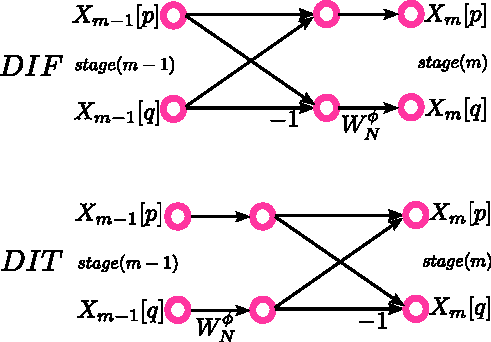
\includegraphics[width=0.65\linewidth]{Diagramas/miSeccionFiguras/DifDit.pdf}
	\caption{Basic butterflies computation in the decimation in time and frequency.}
	\label{fig:difdit}
\end{figure}

In addition, the input samples in FFT algorithms DIF are organized in natural order but its output has not in order, in this case is necessary a circuit for reordering the output data. On the other hand, FFT algorithms DIT is all the  opposite, It has not its input in order and its output has a natural order.

Fallowing the methodology presented in \cite{proakis_digital_nodate}, we can understand and apply the mathematical expressions of \textit{radix-}$2^3$ DIF explained in \cite{jia_efficient_nodate}. 

These fundamental equations are:
\begin{align}\label{eqn:radix}
C_{8k+0} = \sum_{n=0}^{N/8-1} \bigg\{&[(x_n + x_{n+\frac{N}{2}}) + (x_{n+\frac{N}{4}} + x_{n+\frac{3N}{4}})] + 	   				    \\
&[(x_{n+\frac{N}{8}} + x_{n+\frac{5N}{8}}) + (x_{n+\frac{3N}{8}} + x_{n+\frac{7N}{8}})] \bigg\} W_N^{0n} W_{N/8}^ {nk}     \nonumber\\
%	
C_{8k+4} = \sum_{n=0}^{N/8-1} \bigg\{&[(x_n + x_{n+\frac{N}{2}}) + (x_{n+\frac{N}{4}} + x_{n+\frac{3N}{4}})] - 			   \nonumber\\
&[(x_{n+\frac{N}{8}} + x_{n+\frac{5N}{8}}) + (x_{n+\frac{3N}{8}} + x_{n+\frac{7N}{8}})] \bigg\} W_N^{4n} W_{N/8}^ {nk}     \nonumber\\
%
C_{8k+2} = \sum_{n=0}^{N/8-1} \bigg\{&[(x_n + x_{n+\frac{N}{2}}) - (x_{n+\frac{N}{4}} + x_{n+\frac{3N}{4}})] -j 		   \nonumber\\
&[(x_{n+\frac{N}{8}} + x_{n+\frac{5N}{8}}) - (x_{n+\frac{3N}{8}} + x_{n+\frac{7N}{8}})] \bigg\} W_N^{2n} W_{N/8}^ {nk}     \nonumber\\
%
C_{8k+6} = \sum_{n=0}^{N/8-1} \bigg\{&[(x_n + x_{n+\frac{N}{2}}) - (x_{n+\frac{N}{4}} + x_{n+\frac{3N}{4}})] +j			   \nonumber\\
&[(x_{n+\frac{N}{8}} + x_{n+\frac{5N}{8}}) - (x_{n+\frac{3N}{8}} + x_{n+\frac{7N}{8}})] \bigg\} W_N^{6n} W_{N/8}^ {nk}     \nonumber\\
%
C_{8k+1} = \sum_{n=0}^{N/8-1} \bigg\{&[(x_n - x_{n+\frac{N}{2}}) -j (x_{n+\frac{N}{4}} - x_{n+\frac{3N}{4}})] + W_N^{N/8}  \nonumber\\
&[(x_{n+\frac{N}{8}} - x_{n+\frac{5N}{8}}) -j (x_{n+\frac{3N}{8}} - x_{n+\frac{7N}{8}})] \bigg\} W_N^{n} W_{N/8}^ {nk}     \nonumber\\
%
C_{8k+5} = \sum_{n=0}^{N/8-1} \bigg\{&[(x_n - x_{n+\frac{N}{2}}) -j (x_{n+\frac{N}{4}} - x_{n+\frac{3N}{4}})] - W_N^{N/8}  \nonumber\\
&[(x_{n+\frac{N}{8}} - x_{n+\frac{5N}{8}}) -j (x_{n+\frac{3N}{8}} - x_{n+\frac{7N}{8}})] \bigg\} W_N^{5n} W_{N/8}^ {nk}    \nonumber\\
%
C_{8k+3} = \sum_{n=0}^{N/8-1} \bigg\{&[(x_n - x_{n+\frac{N}{2}}) +j (x_{n+\frac{N}{4}} - x_{n+\frac{3N}{4}})] + W_N^{3N/8} \nonumber\\
&[(x_{n+\frac{N}{8}} - x_{n+\frac{5N}{8}}) +j (x_{n+\frac{3N}{8}} - x_{n+\frac{7N}{8}})] \bigg\} W_N^{3n} W_{N/8}^ {nk}    \nonumber\\
%
C_{8k+7} = \sum_{n=0}^{N/8-1} \bigg\{&[(x_n - x_{n+\frac{N}{2}}) +j (x_{n+\frac{N}{4}} + x_{n+\frac{3N}{4}})] - W_N^{3N/8} \nonumber\\
&[(x_{n+\frac{N}{8}} - x_{n+\frac{5N}{8}}) +j (x_{n+\frac{3N}{8}} - x_{n+\frac{7N}{8}})] \bigg\} W_N^{7n} W_{N/8}^ {nk}    \nonumber 	
\end{align}
In Fig. \ref{fig:8puntosradix8conexion} and Fig. \ref{fig:8puntosradix8burbujas} we represent the equivalent diagram of interconnections and data flows from the equations presented in (\ref{eqn:radix}).

The use of higher value radices lead to different amount of rotators. If we compare the quantity of rotators of an architecture \textit{radix-}$2$ FFT with an architecture \textit{radix-}$2^k$ FFT, this last has less number of phase factors than use a \textit{radix-}$2$.
\\

\begin{figure}[!t]
	\centering
	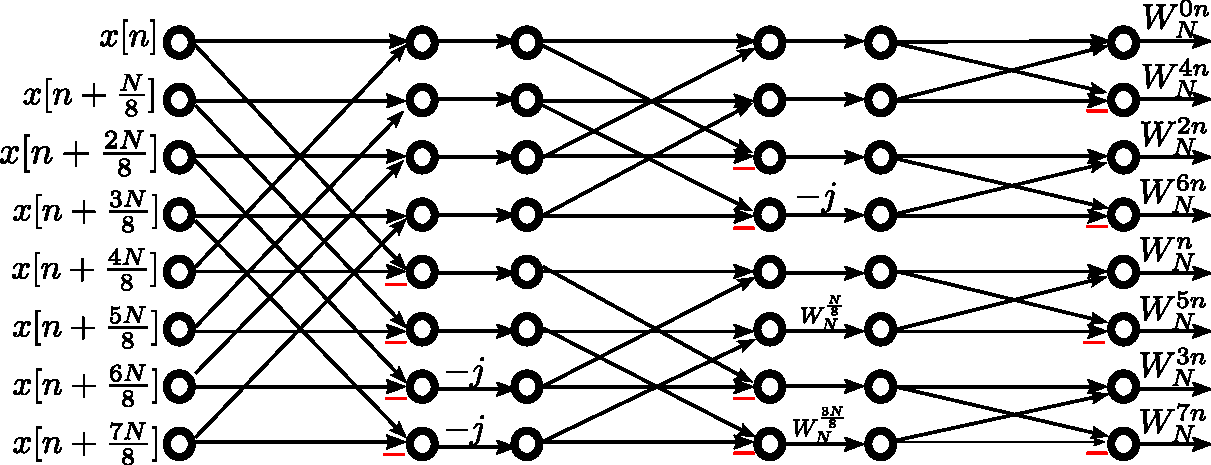
\includegraphics[width=\linewidth]{Diagramas/miSeccionFiguras/8PuntosRadix8Conexion.pdf}
	\caption{Structure of interconnection for \textit{radix-}$2^3$ DIF DFT}
	\label{fig:8puntosradix8conexion}
\end{figure}
\begin{figure}[t!]
	\centering
	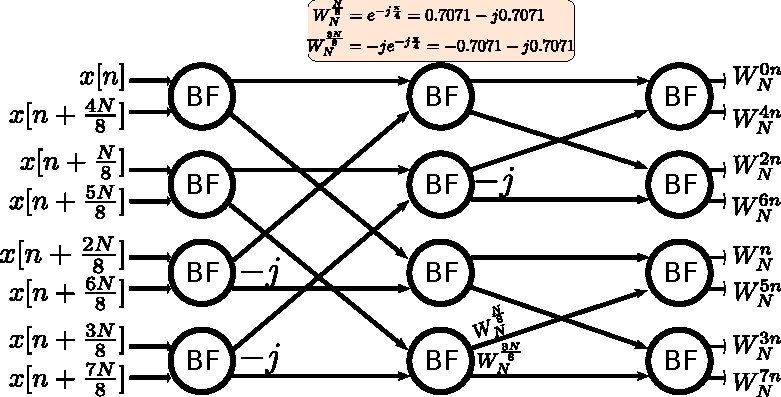
\includegraphics[width=0.95\linewidth]{Diagramas/miSeccionFiguras/8PuntosRadix8Burbujas.pdf}
	\caption{Data flow graph (DFG) based in equations (\ref{eqn:radix}).}
	\label{fig:8puntosradix8burbujas}
\end{figure}
\begin{figure}[t!]
	\centering
	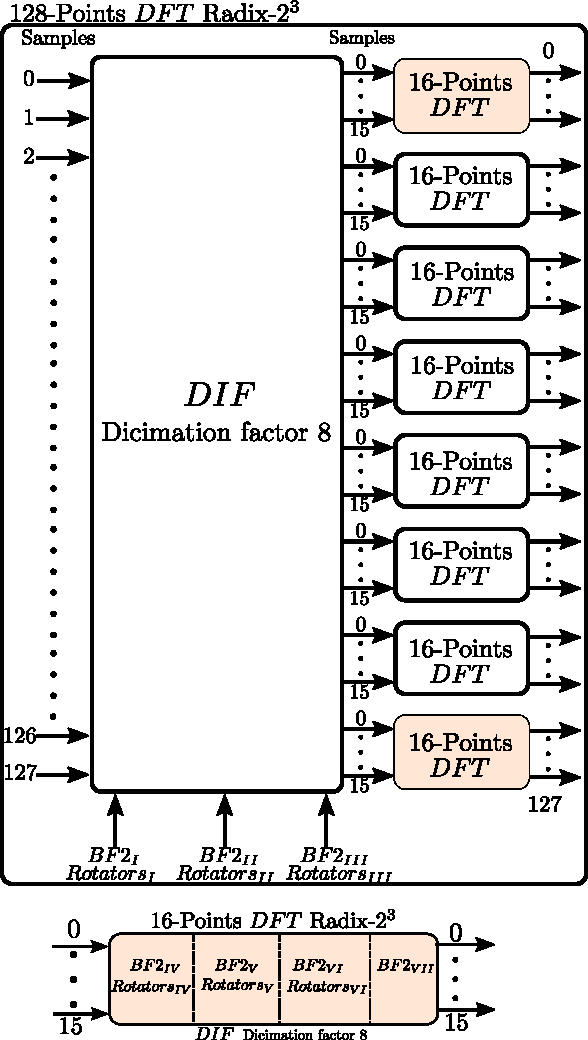
\includegraphics[width=0.8\linewidth]{Diagramas/miSeccionFiguras/BloquesDft.pdf}
	\caption{Decomposing a \textit{radix-}$2^3$ 128-point DFT	}
	\label{fig:bloquesdft}
\end{figure}
With these first approaches, we are in conditions to design a $128$-$points$ DFT \textit{radix-}$2^3$. Applying the divide and conquer strategy by decomposition of a 128-point DFT in smaller DFTs. We begin to apply the set of equations (\ref{eqn:radix}) for the 128 point DFT and calculating each coefficient $C_{8k+i} = \sum_{n=0}^{128/8-1} \{ \cdot \}, $ for $k=0,1,...,(128/8)-1$. In this way we get a sequence in chain of butterflies with its corresponding rotation factor and the correct index of the samples in witch them must be added or multiplied. This technique lets us do a subdivision on butterflies' stages, in Fig. \ref{fig:bloquesdft} we can see that the 128 point DFT goes through a processes that involve tree stages of butterflies to arrive finally to a set of eight DFT where each of one is a 16 point DFT.

The next step to can calculate finally our 128 point DFT is to find the suitable rotator factors for the 16 point DFT, this process follow exactly the same calculation that we comment and remark previously, the use of the above equations (\ref{eqn:radix}) are essential for this design and them are evaluated to get $C_{8k+i} = \sum_{n=0}^{16/8-1} \{ \cdot \}, $ for $k=0,1$. The structure for the 16 point DFT is described in Fig. \ref{fig:16puntosradix8conexion} and Fig. \ref{fig:16puntosradix8burbujas}. 
\begin{figure}[h!]
	\centering
	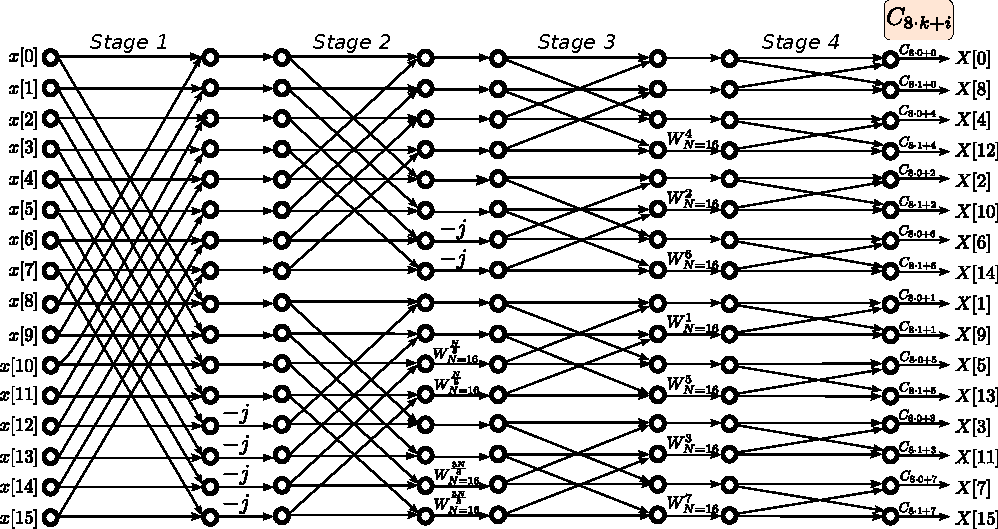
\includegraphics[width=\linewidth]{Diagramas/miSeccionFiguras/16PuntosRadix8Conexion.pdf}
	\caption{Flow graph of a \textit{radix-}$2^3$ 16-point DIF DFT}
	\label{fig:16puntosradix8conexion}
\end{figure}
\begin{figure}[h!]
	\centering
	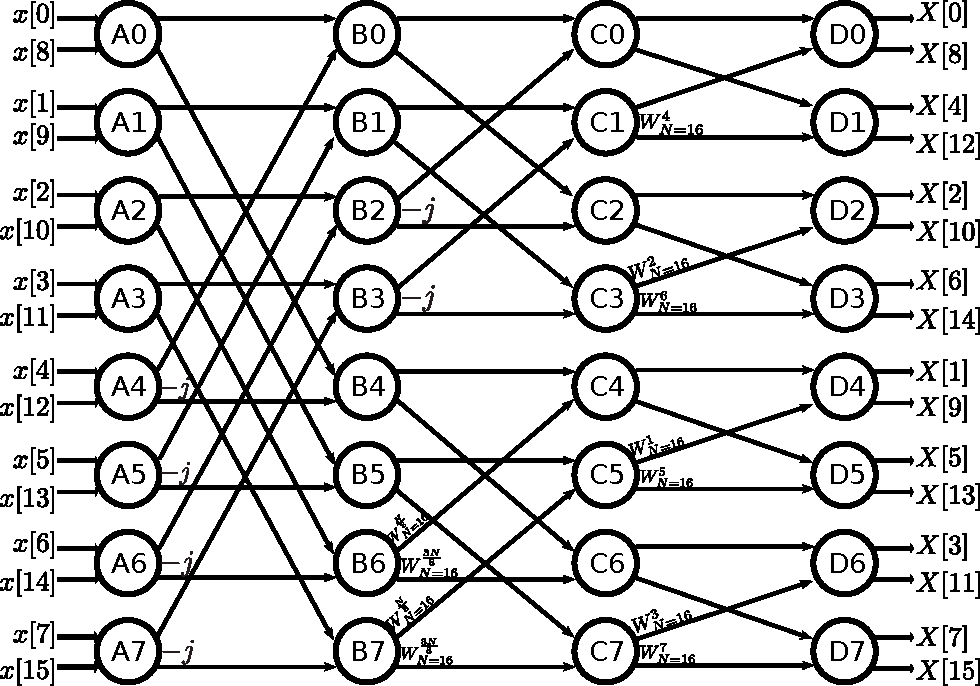
\includegraphics[width=\linewidth]{Diagramas/miSeccionFiguras/16PuntosRadix8Burbujas.pdf}
	\caption{Data flow graph (DFG) for a \textit{radix-}$2^3$ 16-point DIF DFT}
	\label{fig:16puntosradix8burbujas}
\end{figure}

With the DFT's previous decomposition we learned how to get whole the coefficients $C_{8k+i}$ that represent the samples in frequency $X[k]$ obtained from a combination of the different instances of $x[n]$. This method take us to apply step by step the equation (\ref{eqn:radix}) to our design and finally arrive to the definitive architecture, the Fig. \ref{fig:128puntosradix8conexion} shows us a \textit{radix-}$2^3$ 128-point DIF DFT with a total of seven stages where each stage is building with 64 butterflies of radix-2 base.
\begin{figure}[t!]
	\centering
	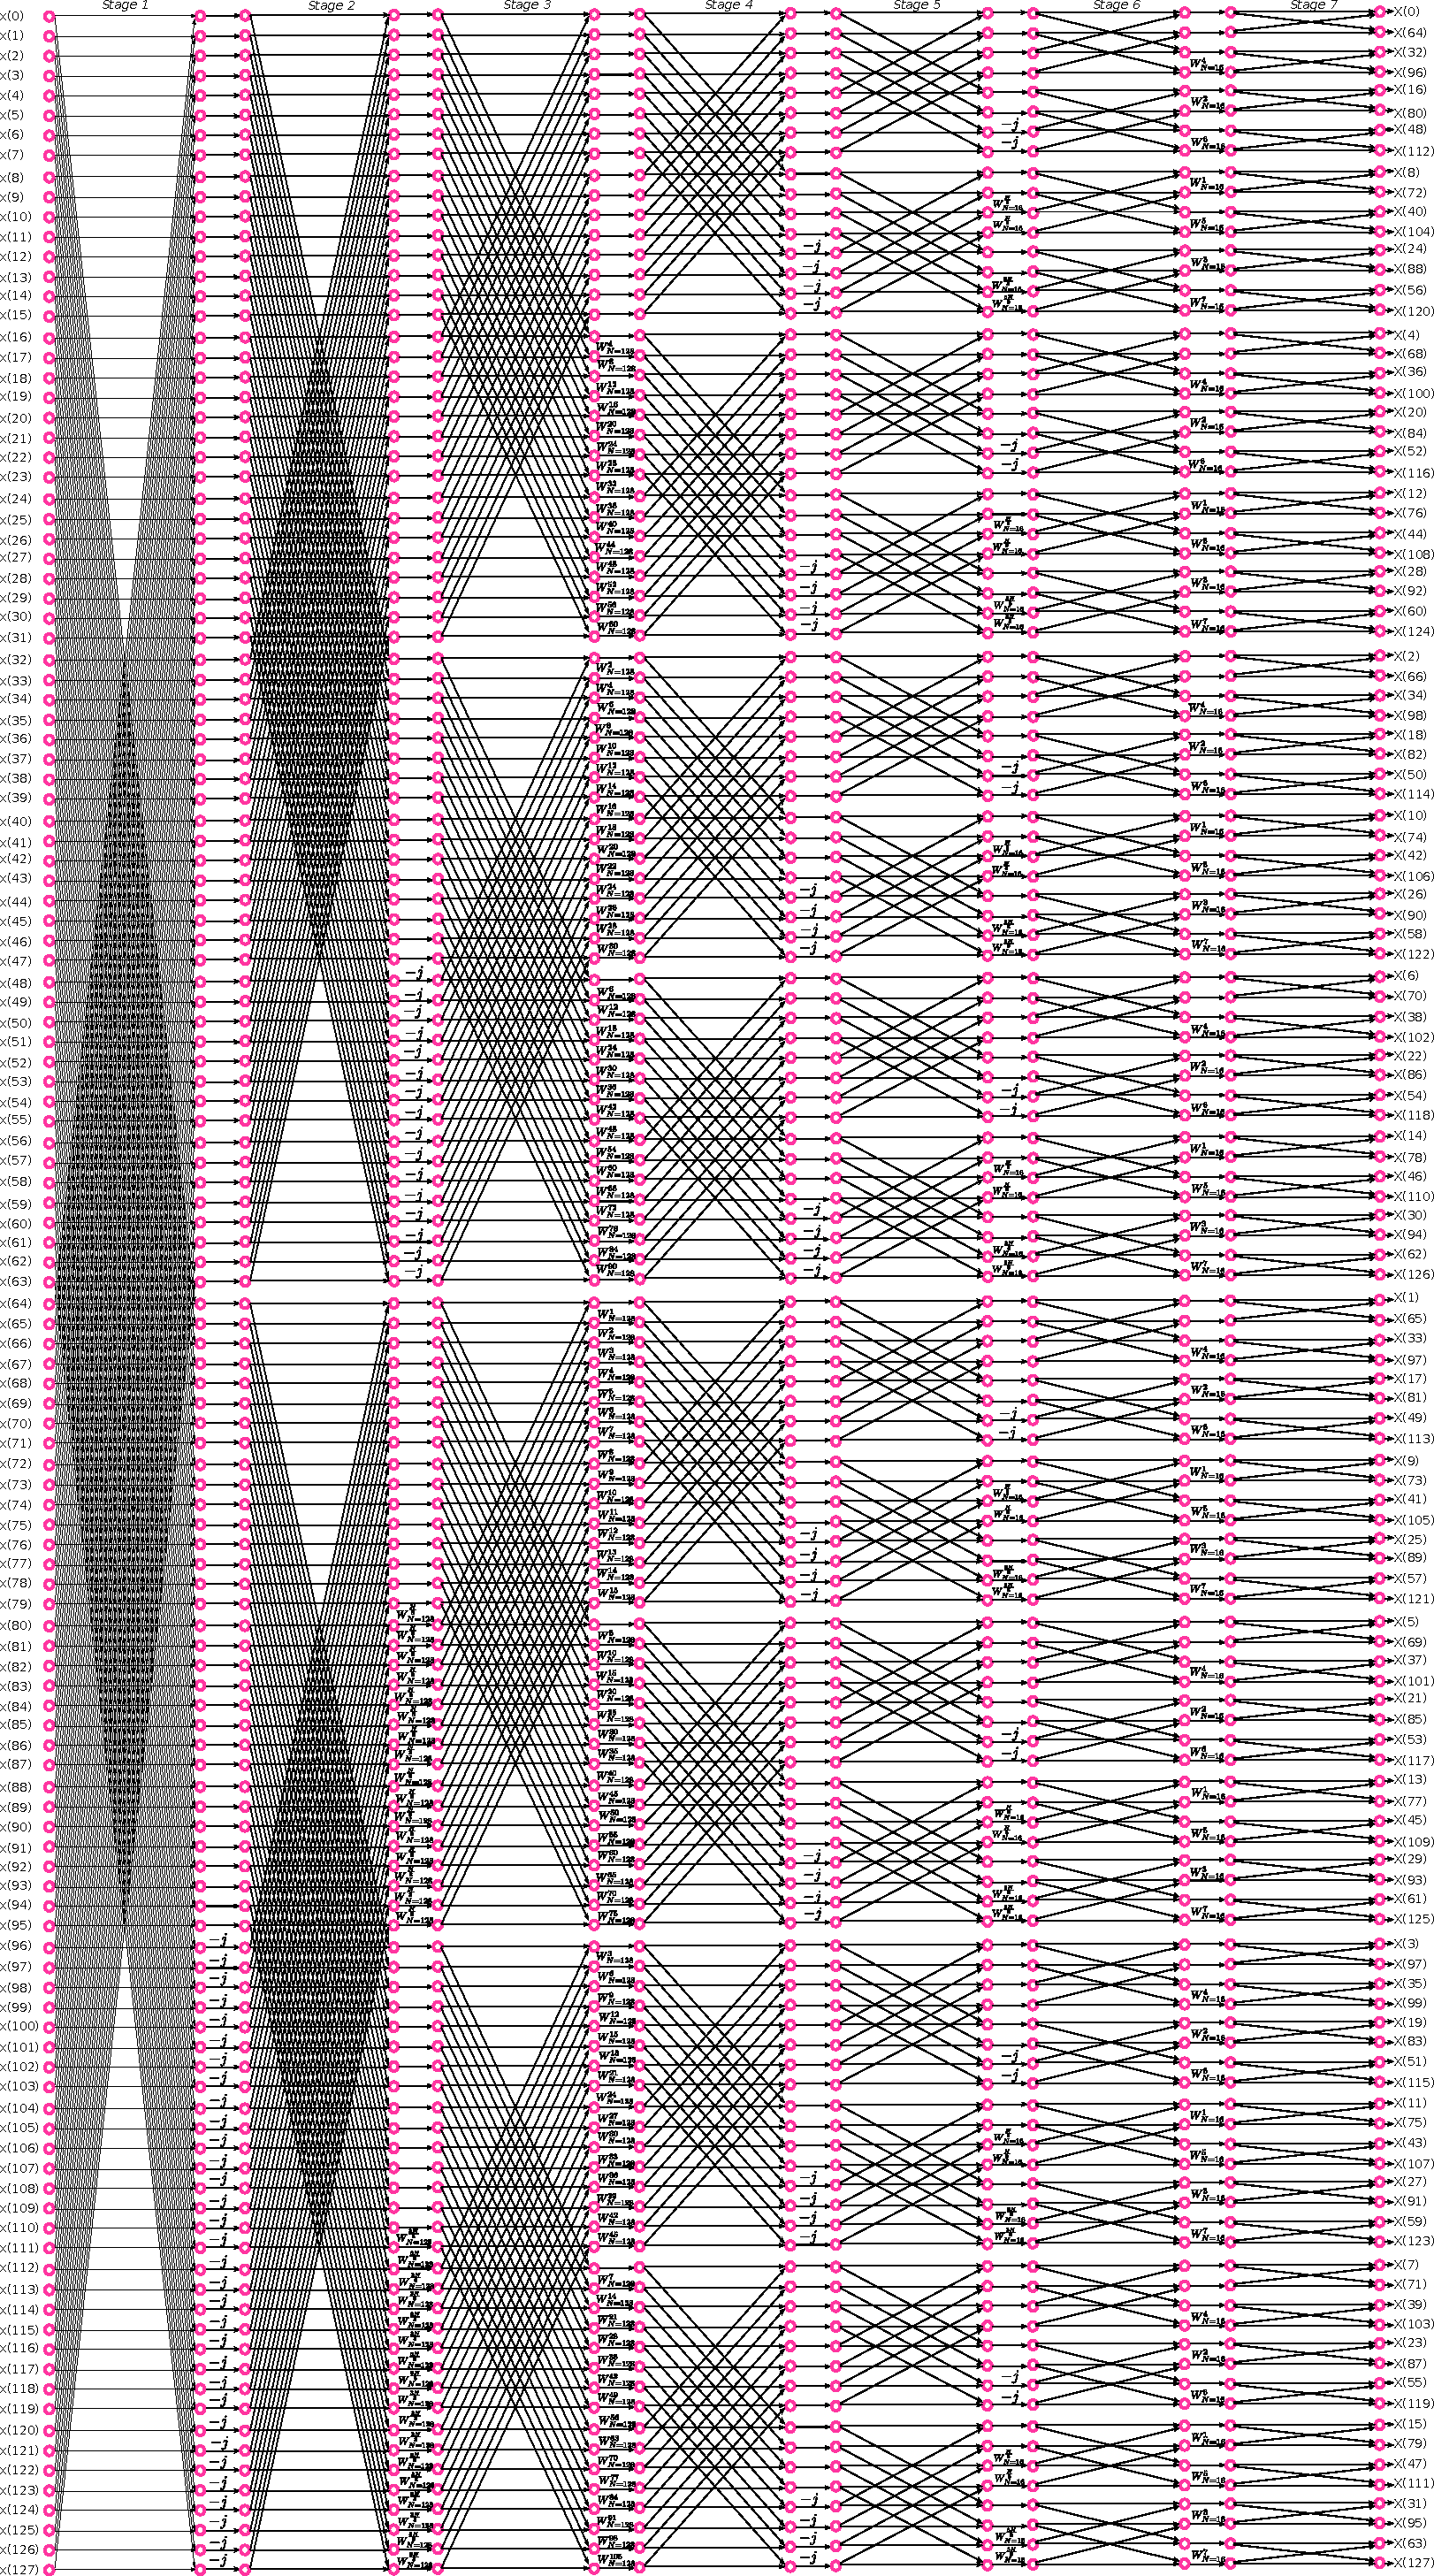
\includegraphics[width=\linewidth]{Diagramas/miSeccionFiguras/128PuntosRadix8Conexion.pdf}
	\caption{Flow graph of a \textit{radix-}$2^3$ 128-point DIF DFT}
	\label{fig:128puntosradix8conexion}
\end{figure}



%%%%%%%%%%
%% Seccion
%%%%%%%%%%
\section{DESIGN OF FFT ARCHITECTURE VIA FOLDING}
In this section, we illustrate the folding transformation method to derive a 16-point DIF FFT 4-parallel architecture as an example and then, using the same method, we extend it to 128-point architecture. To do this, we will use the architecture proposed in \cite{ayinala_pipelined_2012}.
%%%%%%%%%%%%%
%% Subseccion
%%%%%%%%%%%%%
\subsection{4-Parallel radix-$2^3$ 16-Points}
In Fig. \ref{fig:16puntosradix8conexion} we can see the flow graph of a 16-point DIF FFT radix-$2^3$ with main base radix-2. The graph is divided into four stages and each of them consist of a set of butterflies and multipliers. The twiddle factor in between the stages indicates a multiplication by $W^k_N$, where $W_N$ denotes the \textit{N}th root of unity, with its exponent evaluated modulo N. This can be represented as a DFG as shown in Fig. \ref{fig:16puntosradix8burbujas} where the nodes represents the butterfly computations of the radix-2 FFT algorithm. 

The folding transformation is used on the DFG in to derive a pipelined architecture. To do this we need a folding set, which is an ordered set of operations executed by the same functional unit. Each folding set contains K entries, where K is called the folding factor. The operation in the \textit{j}th position within the folding set (where goes from 0 to K-1) is executed by the functional unit during the time partition. The term is called the folding order.

First we need to derive the folding equations, to do this consider an edge $e$ connecting the nodes \textit{U} and \textit{V} with $w(e)$ delays. Let the executions of the \textit{l}th iteration of the nodes \textit{U} and \textit{V} be scheduled at the time units $Kl+u$ and $Kl+v$ respectively, where $u$ and $v$ are the folding orders of the nodes \textit{U} and \textit{V}, respectively. The folding equation for the edge $e$ is:
\begin{equation}\label{eqn:fold_equation}
D_F(U \to V) = Kw(e)-P_U+v-u
\end{equation}

where $P_U$ is the number of pipeline stages in the hardware unit which executes the node U.
Consider folding of the the DFG in Fig. \ref{fig:16puntosradix8burbujas} with the folding sets:
\begin{align*}%\label{eq:foldingset_16}
A&= \{ A0,A2,A4,A6 \}  & A'&= \{ A1,A3,A5,A7 \} \\
B&=\{ B1,B3,B0,B2 \}   &B'&=\{ B5,B7,B4,B6 \} 	\\
C&=\{ C2,C1,C3,C0 \}   &C'&=\{ C6,C5,C7,C4 \} 	\\ 
D&=\{ D3,D0,D2,D1 \}   &D'&=\{ D7,D4,D6,D5 \}  
\end{align*}
Assuming that the butterfly operations do not have any pipeline stages ($P_A=P_B=P_C=P_D=0$), the folding equations can be derived for all edges. Thus, we can obtained from (\ref{eqn:fold_equation}) the expressions \textit{without apply retiming}.
\begin{small}
\begin{align*}
D_F(D0\to B0)&=2 &  D_F(D0\to B4)&=2\\
D_F(D1\to B1)&=0 &  D_F(D1\to B5)&=0\\
D_F(D2\to B2)&=2 &  D_F(D2\to B6)&=2\\
D_F(D3\to B3)&=-1& D_F(D3\to B7)&=-1\\
D_F(D4\to B0)&=0 &  D_F(D4\to B4)&=0\\
D_F(D5\to B1)&=-1& D_F(D5\to B5)&=-1\\
D_F(D6\to B2)&=0 &  D_F(D6\to B6)&=0\\
D_F(D7\to B3)&=-2& D_F(D7\to B7)&=-2\\
D_F(E0\to C0)&=1 &  D_F(E0\to C2)&=-2\\
D_F(E1\to C1)&=1 &  D_F(E1\to C3)&=2\\
D_F(E2\to C0)&=0 &  D_F(E2\to C2)&=-3\\
D_F(E3\to C1)&=0 &  D_F(E3\to C3)&=1\\
D_F(E4\to C4)&=1 &  D_F(E4\to C6)&=-2\\
D_F(E5\to C5)&=1 &  D_F(E5\to C7)&=2\\
D_F(E6\to C4)&=0 &  D_F(E6\to C6)&=-3\\
D_F(E7\to C5)&=0 &  D_F(E7\to C7)&=1\\
D_F(F0\to D0)&=-2& D_F(F0\to D1)&=0\\
D_F(F1\to D0)&=0 &  D_F(F1\to D1)&=2\\
D_F(F2\to D2)&=2 &  D_F(F2\to D3)&=0\\
D_F(F3\to D2)&=0 &  D_F(F3\to D3)&=-2\\
D_F(F4\to D4)&=-2&  D_F(F4\to D5)&=0\\
D_F(F5\to D4)&=0 &  D_F(F5\to D5)&=2\\
D_F(F6\to D6)&=2 &  D_F(F6\to D7)&=0\\
D_F(F7\to D6)&=0 &  D_F(F7\to D7)&=-2
\end{align*}
\end{small}
For the folded system to be realizable, $D_F(U\to V)\geq0$ must hold for all the edges in the DFG. Retimming and/or pipeline can be applied to satisfy this property, if the DFG in Fig. \ref{fig:16puntosradix8burbujas} is pipelined/retimmed as shown in Fig. \ref{fig:dfg_16_ret} the system is realizable and the folded delays for the edges are given by the equations that represent a folding set \textit{with retiming}
\begin{figure}[h!]
\centering
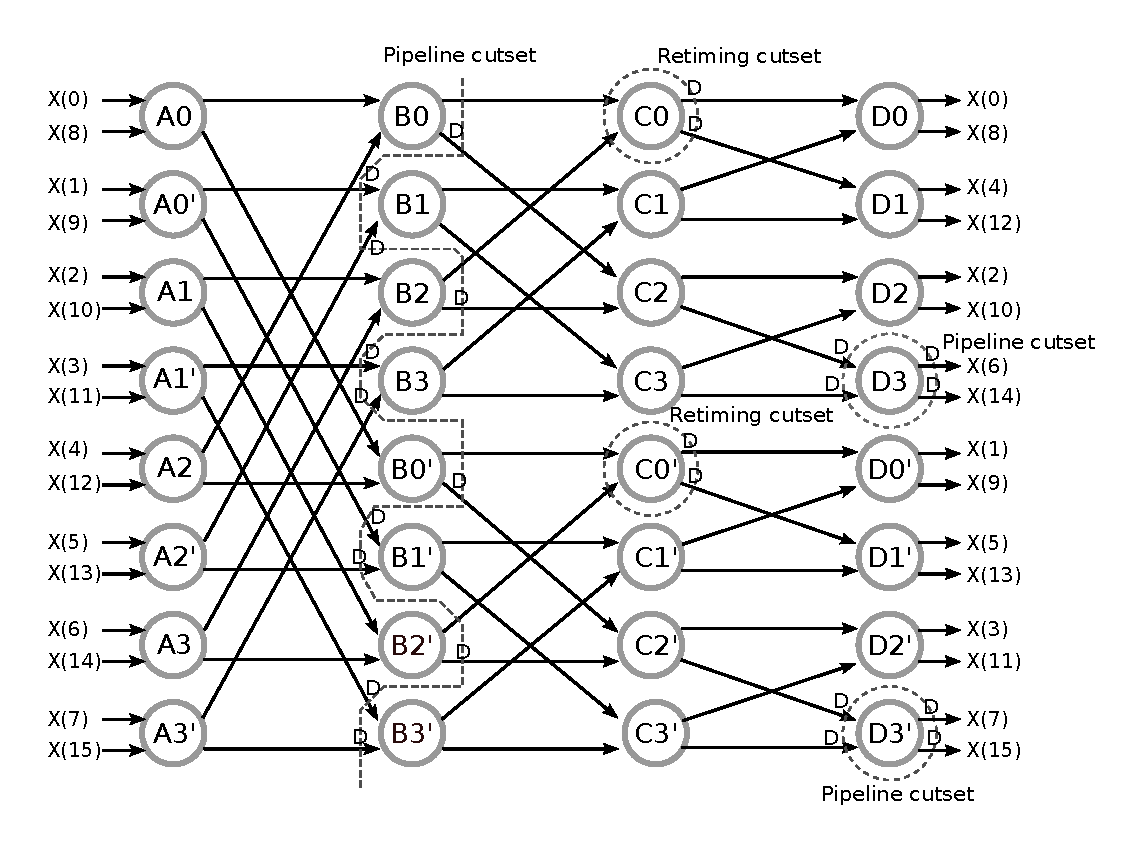
\includegraphics[width=\linewidth]{Diagramas/Butter16_pipe.eps}
\caption{Data Flow graph (DFG) of a radix-2 16-point DIF FFT with retiming and pipeline.}
\label{fig:dfg_16_ret}
\end{figure}
\begin{small}
\begin{align}\label{eqn:ConRetiming} 
D_F(D0\to B0)&=2 &  D_F(D0\to B4)&=2 		 \\
D_F(D1\to B1)&=4 &  D_F(D1\to B5)&=4\nonumber\\
D_F(D2\to B2)&=2 &  D_F(D2\to B6)&=2\nonumber\\
D_F(D3\to B3)&=3 &  D_F(D3\to B7)&=3\nonumber\\
D_F(D4\to B0)&=0 &  D_F(D4\to B4)&=0\nonumber\\
D_F(D5\to B1)&=3 &  D_F(D5\to B5)&=3\nonumber\\
D_F(D6\to B2)&=0 &  D_F(D6\to B6)&=0\nonumber\\
D_F(D7\to B3)&=2 &  D_F(D7\to B7)&=2\nonumber\\
D_F(E0\to C0)&=1 &  D_F(E0\to C2)&=2\nonumber\\
D_F(E1\to C1)&=1 &  D_F(E1\to C3)&=2\nonumber\\
D_F(E2\to C0)&=0 &  D_F(E2\to C2)&=1\nonumber\\
D_F(E3\to C1)&=0 &  D_F(E3\to C3)&=1\nonumber\\
D_F(E4\to C4)&=1 &  D_F(E4\to C6)&=2\nonumber\\
D_F(E5\to C5)&=1 &  D_F(E5\to C7)&=2\nonumber\\
D_F(E6\to C4)&=0 &  D_F(E6\to C6)&=1\nonumber\\
D_F(E7\to C5)&=0 &  D_F(E7\to C7)&=1\nonumber\\
D_F(F0\to D0)&=2 &  D_F(F0\to D1)&=4\nonumber\\
D_F(F1\to D0)&=0 &  D_F(F1\to D1)&=2\nonumber\\
D_F(F2\to D2)&=2 &  D_F(F2\to D3)&=4\nonumber\\
D_F(F3\to D2)&=0 &  D_F(F3\to D3)&=2\nonumber\\
D_F(F4\to D4)&=2 &  D_F(F4\to D5)&=4\nonumber\\
D_F(F5\to D4)&=0 &  D_F(F5\to D5)&=2\nonumber\\
D_F(F6\to D6)&=2 &  D_F(F6\to D7)&=4\nonumber\\
D_F(F7\to D6)&=0 &  D_F(F7\to D7)&=2\nonumber
\end{align}
\end{small}
We can see that the number of register required to implement the folding equations in (\ref{eqn:ConRetiming}) is 80. For minimize the number of registers we use the register minimization technique. 
If we let the output of node A1 be $y_{(0)}$ and $y_{(8)}$, applying this successively with the rest of the nodes A we can obtain the linear life time chart for this stage in Fig. \ref{fig:tab-life-a}. Applying this criteria to the rest of the stages we can obtain the life time chart \ref{fig:tab-life-b} and \ref{fig:tab-life-c} for the outputs of the nodes B and C respectively, we can see that the numbers of maximum registers in each stage are 8, 4 and 8 respectively. More information about this method can be found on \cite{pipeline_parhi_book}.
\begin{figure}[t!]
\centering
 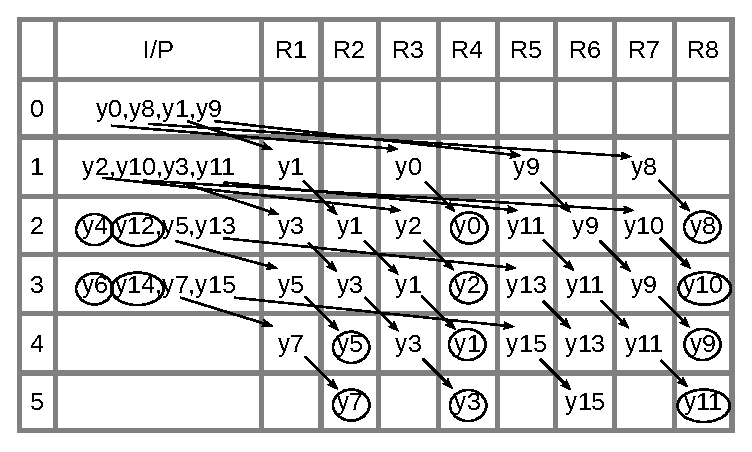
\includegraphics[width=0.9\linewidth]{Diagramas/tab_life_a.eps}
\caption{Linear lifetime chart for the variables $y_{(0)}, y_{(1)},...,y_{(15)}$ for a 16-point FFT architecture.}
\label{fig:tab-life-a}
\end{figure}
\begin{figure}[t!]
\centering
 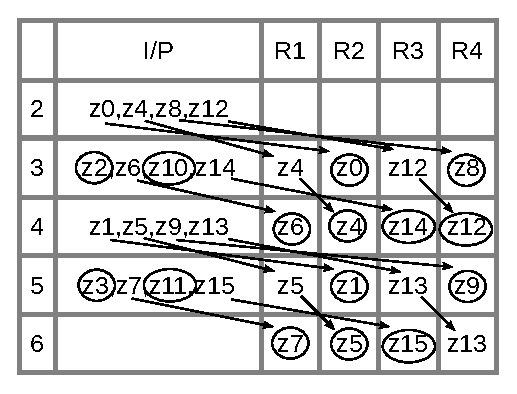
\includegraphics[width=0.63\linewidth]{Diagramas/tab_life_b.eps}
\caption{Linear lifetime chart for the variables $z_{(0)}, z_{(1)},...,z_{(15)}$ for a 16-point FFT architecture.}
\label{fig:tab-life-b}
\end{figure}
\begin{figure}[t!]
\centering
 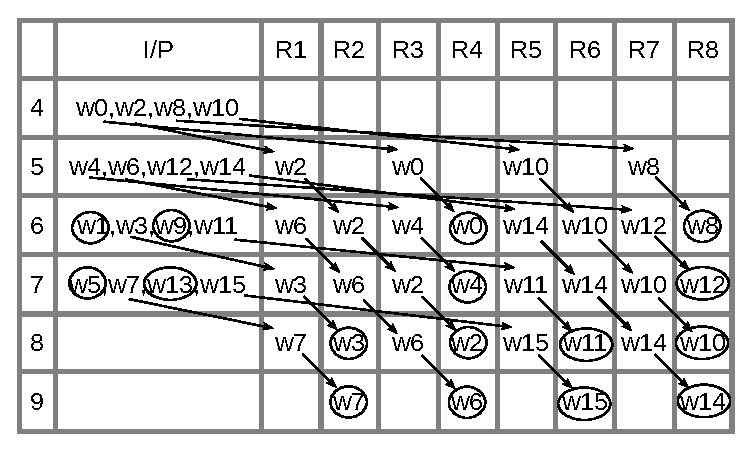
\includegraphics[width=0.95\linewidth]{Diagramas/tab_life_c.eps}
\caption{Linear lifetime chart for the variables $w_{(0)}, w_{(1)},...,w_{(15)}$ for a 16-point FFT architecture.}
\label{fig:tab-life-c}
\end{figure}
The register allocation tables for each of lifetime charts are shown in Fig. \ref{fig:tab-aloc-a}, \ref{fig:tab-aloc-b} and \ref{fig:tab-aloc-c} respectively, we can implement the same equations in (\ref{eqn:ConRetiming}) using 20 registers with register minimization techniques. The folded architecture in Fig. \ref{fig:circ-folding-16} is synthesized using the folding equations and the register allocation tables, the method can be found in \cite{pipeline_parhi_book}. 

The inputs of each folding node are represented with a matrix where the values in the same column are data that flow in parallel and values in the same row
flow through the same path in consecutive clock cycles. The first two rows represents the inputs of the superior BF and the others two represents the input of the inferior BF. 
The same criteria is used for represent the constants of rotators, where each number $k$ of the matrix represent a multiplication by $W^k_N$.
\begin{figure}[!t]
\centering
 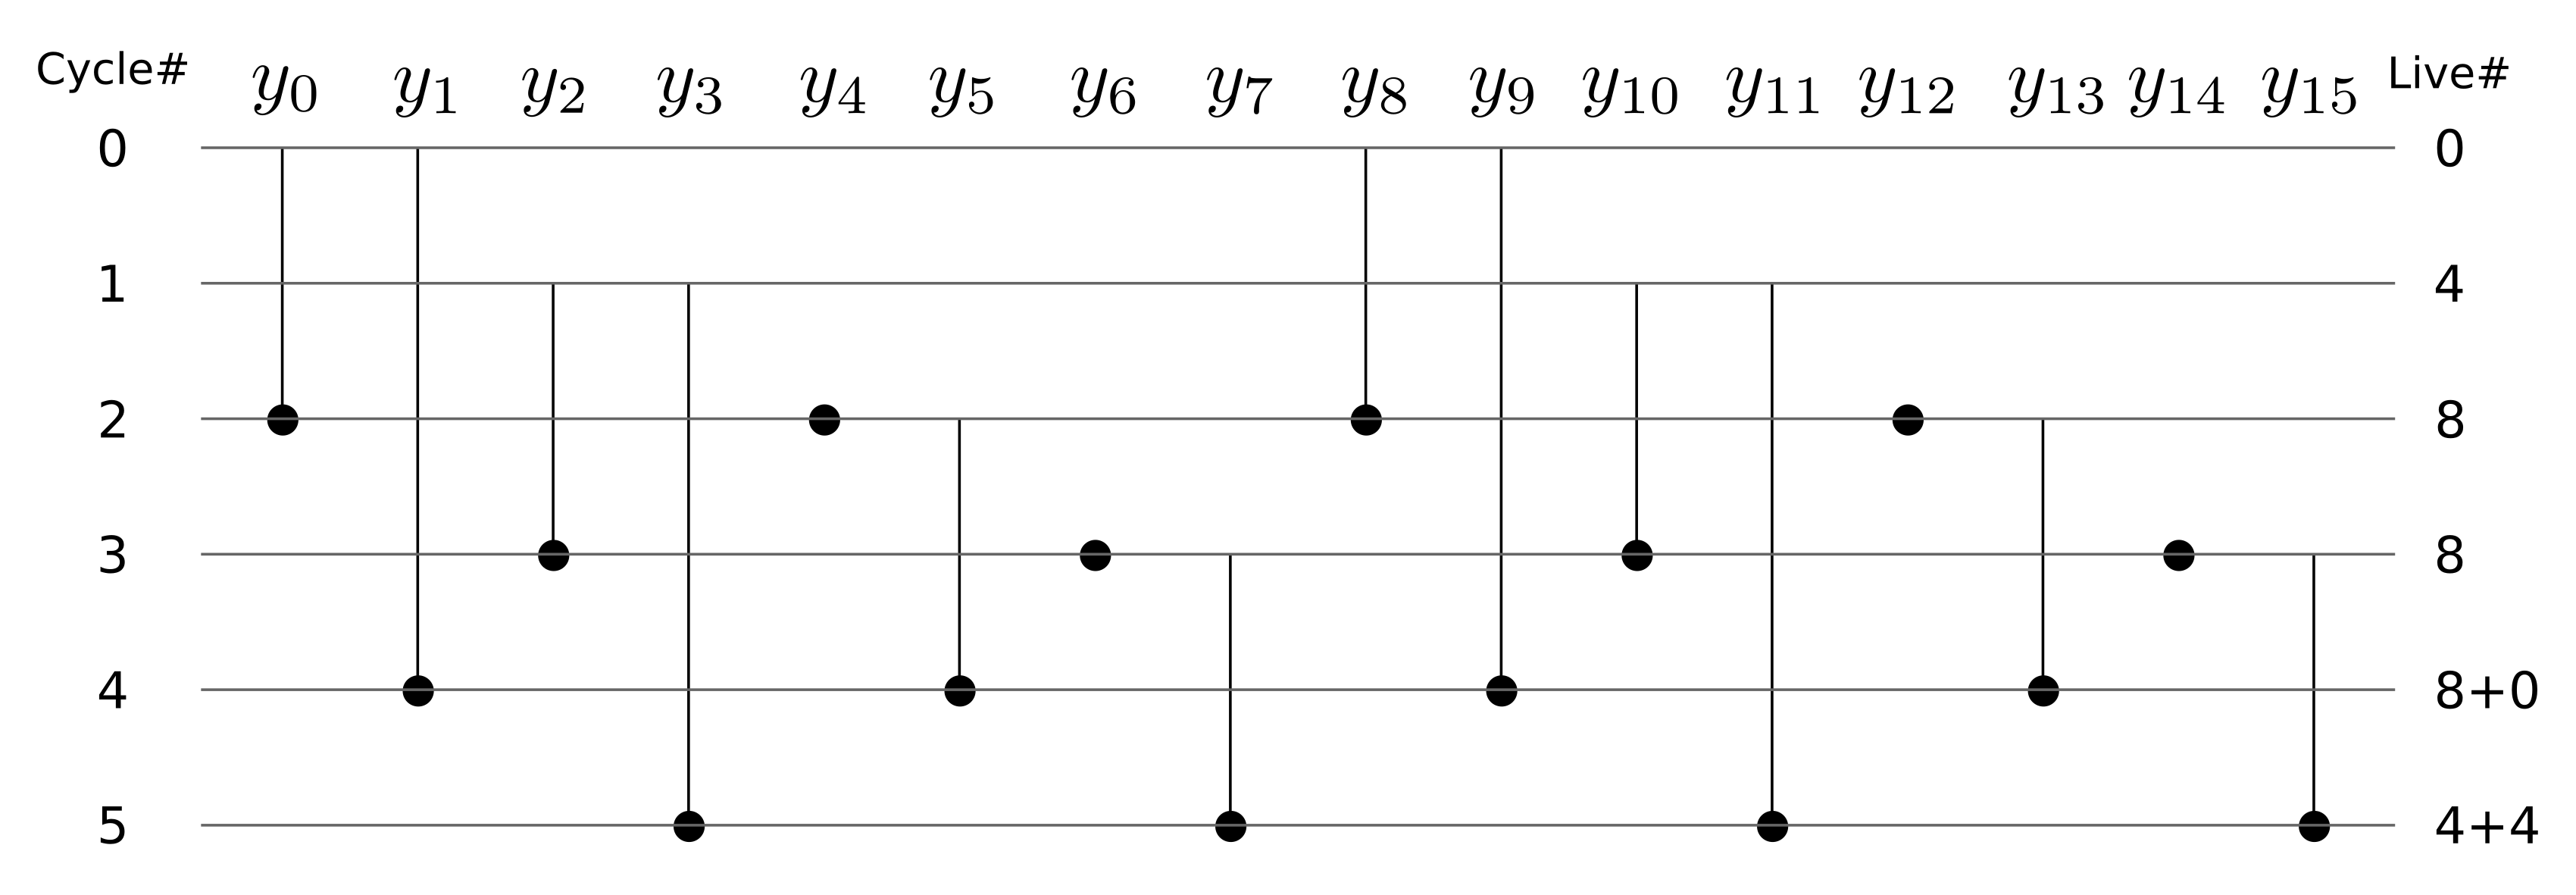
\includegraphics[width=0.95\linewidth]{Diagramas/life_chart_a.png}
\caption{Register allocation table for the data represented in \ref{fig:tab-life-a}}
\label{fig:tab-aloc-a}
\end{figure}
\begin{figure}[!t]
\centering
 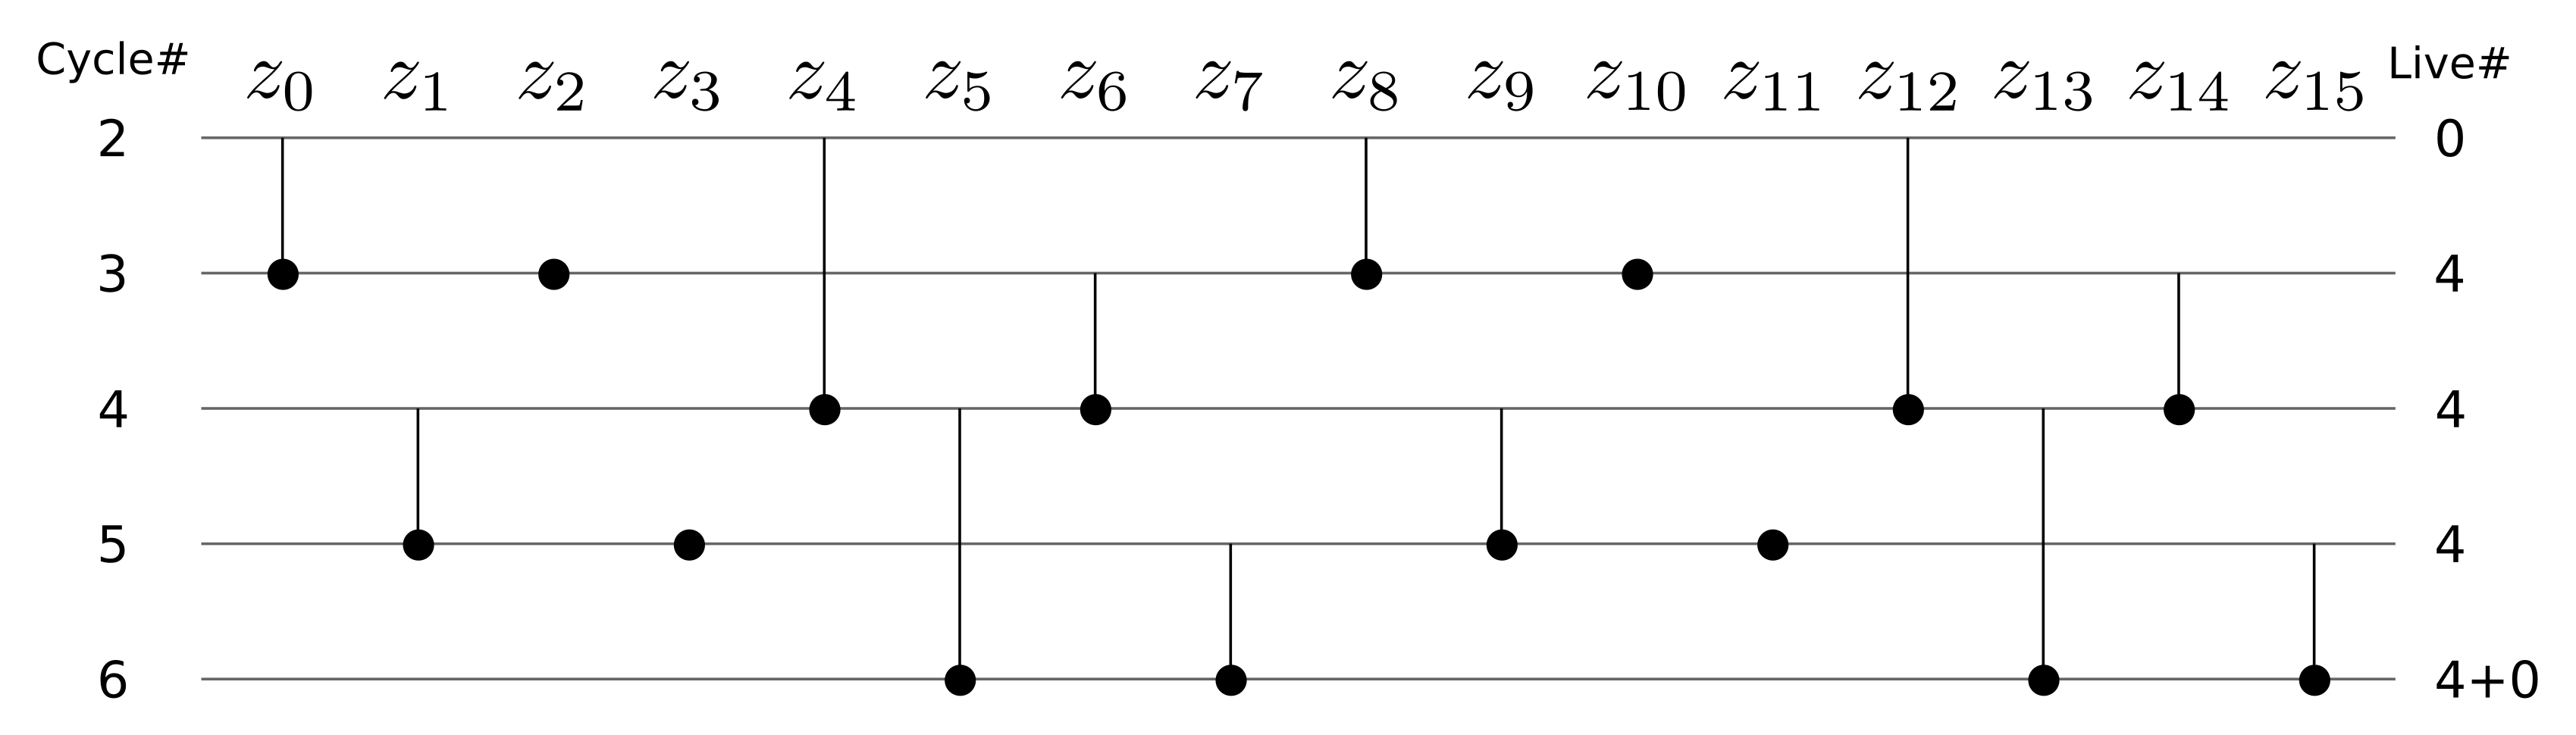
\includegraphics[width=0.95\linewidth]{Diagramas/life_chart_b.png}
\caption{Register allocation table for the data represented in \ref{fig:tab-life-b}}
\label{fig:tab-aloc-b}
\end{figure}
\begin{figure}[!t]
\centering
 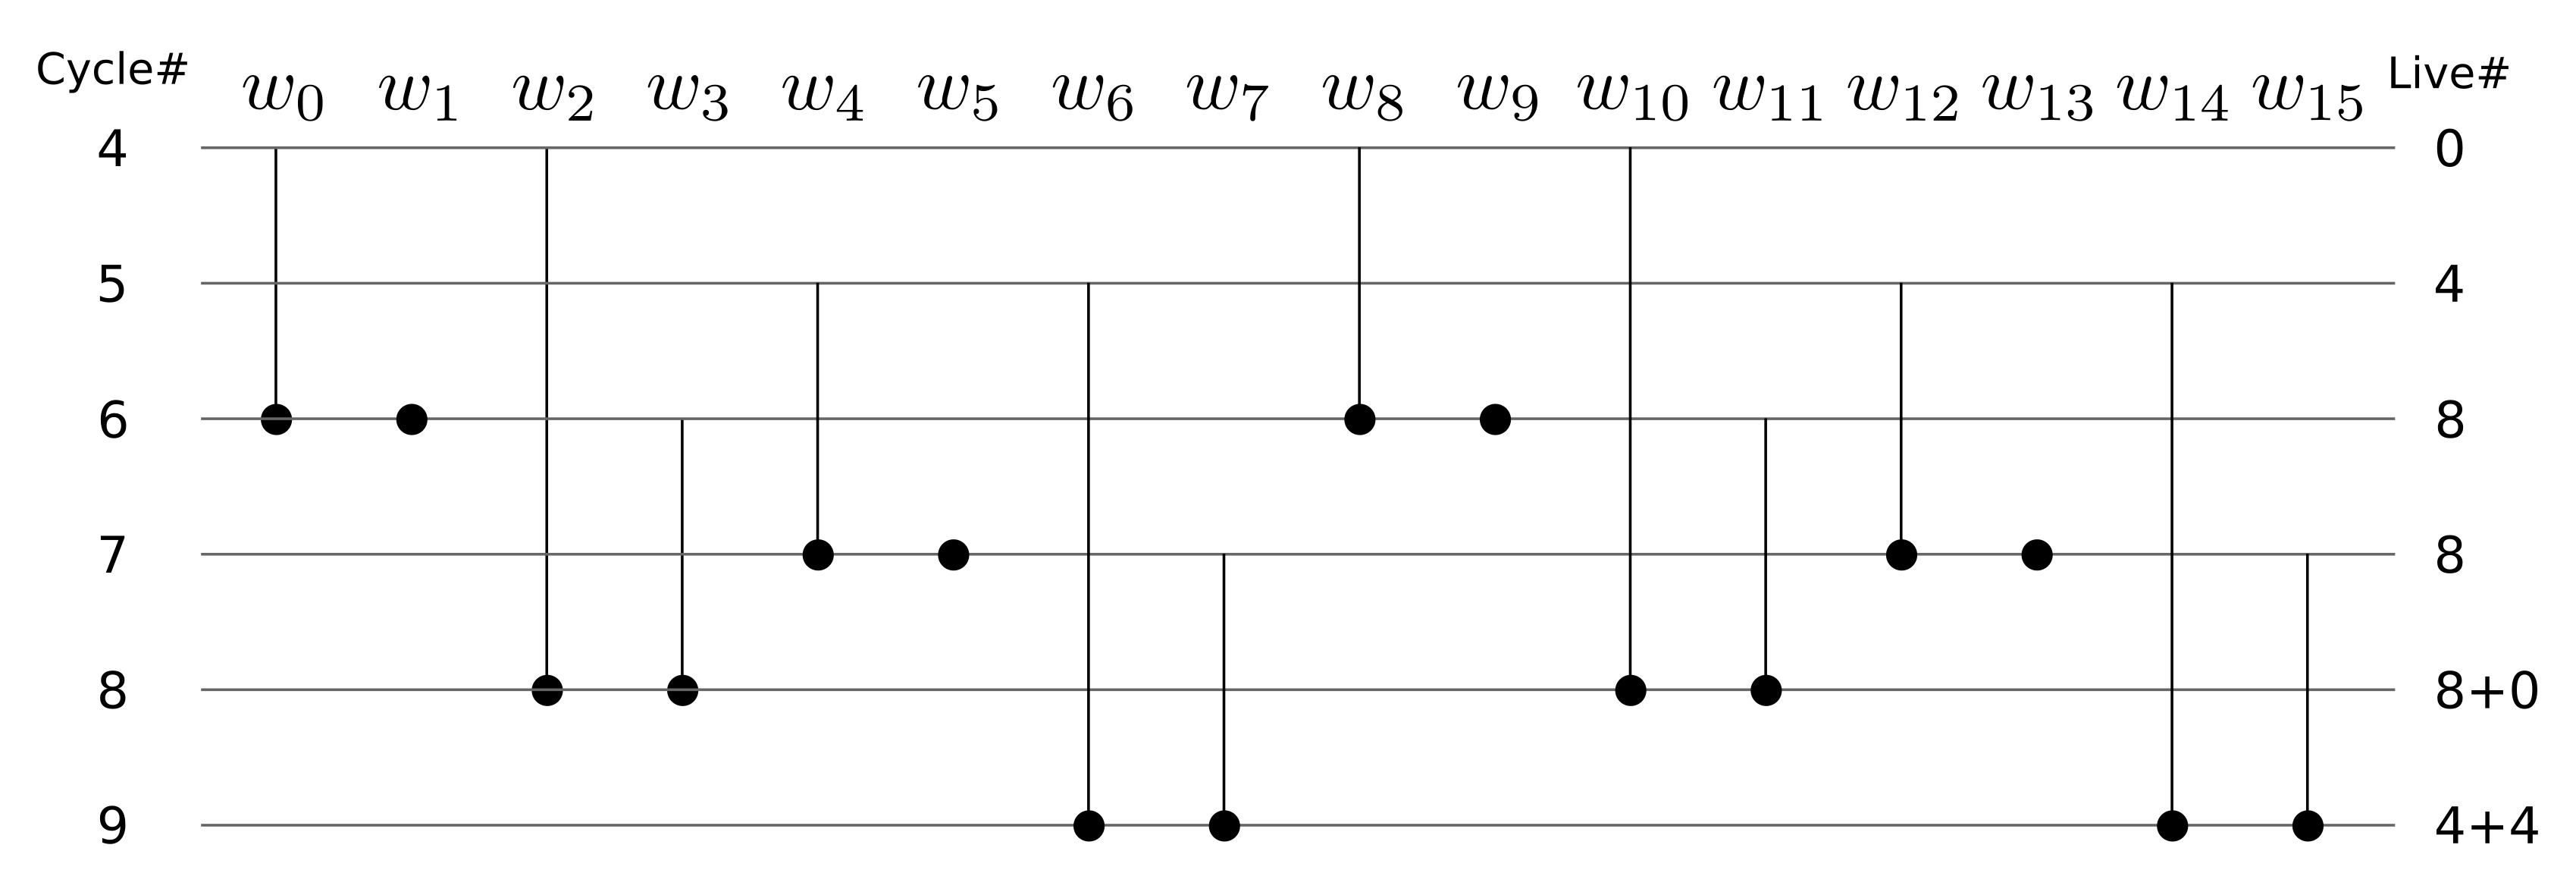
\includegraphics[width=0.95\linewidth]{Diagramas/life_chart_c.png}
\caption{Register allocation table for the data represented in \ref{fig:tab-life-c}}
\label{fig:tab-aloc-c}
\end{figure}
As we can see in Fig. \ref{fig:circ-folding-16}, we suppose that the inputs and output are not ordered, to order these variables extra logic are needed, using more registers and multiplexers.

The different types of rotators used in Fig. \ref{fig:circ-folding-16} are shown in Fig. \ref{fig:rotators}, the description of each of them can be found below.
\begin{itemize}
	\item Trivial rotator: They can be carried out by interchanging the real and imaginary components and/or changing the sign of the data.
	\item Constant CSD rotator: They can be carried out by interchanging the real and imaginary components and/or a multiplication by a unique constant fractional number, in this case we will use a CSD multiplier to perform the area utilized.
	\item General rotator: They can be carried out by interchanging the real and imaginary components and/or a multiplication by more than one constant fractional numbers, in this case we will use a general multiplier.
\end{itemize}
\begin{figure}[h!]
	\centering
	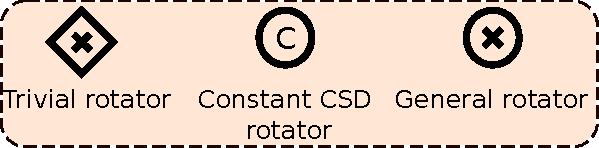
\includegraphics[width=0.6\linewidth]{Diagramas/miSeccionFiguras/Rotadores.pdf}
	\caption{Symbols used for the different types of rotators}
	\label{fig:rotators}
\end{figure}



%%%%%%%%%%%%%
%% Subseccion
%%%%%%%%%%%%%
\subsection{4-Parallel radix-$2^3$ 128-Points}
We can deduce the folding architecture following the same method than used with the 4-Parallel radix-$2^3$ 16-Points. The DFG and folding set used can be shown in Fig. \ref{fig:pipe_dfg_128} and Table \ref{tab:fold_set_128}.
The architecture can be seen in Fig. \ref{fig:circ-folding-128}.
\begin{figure}[t!]
\centering
 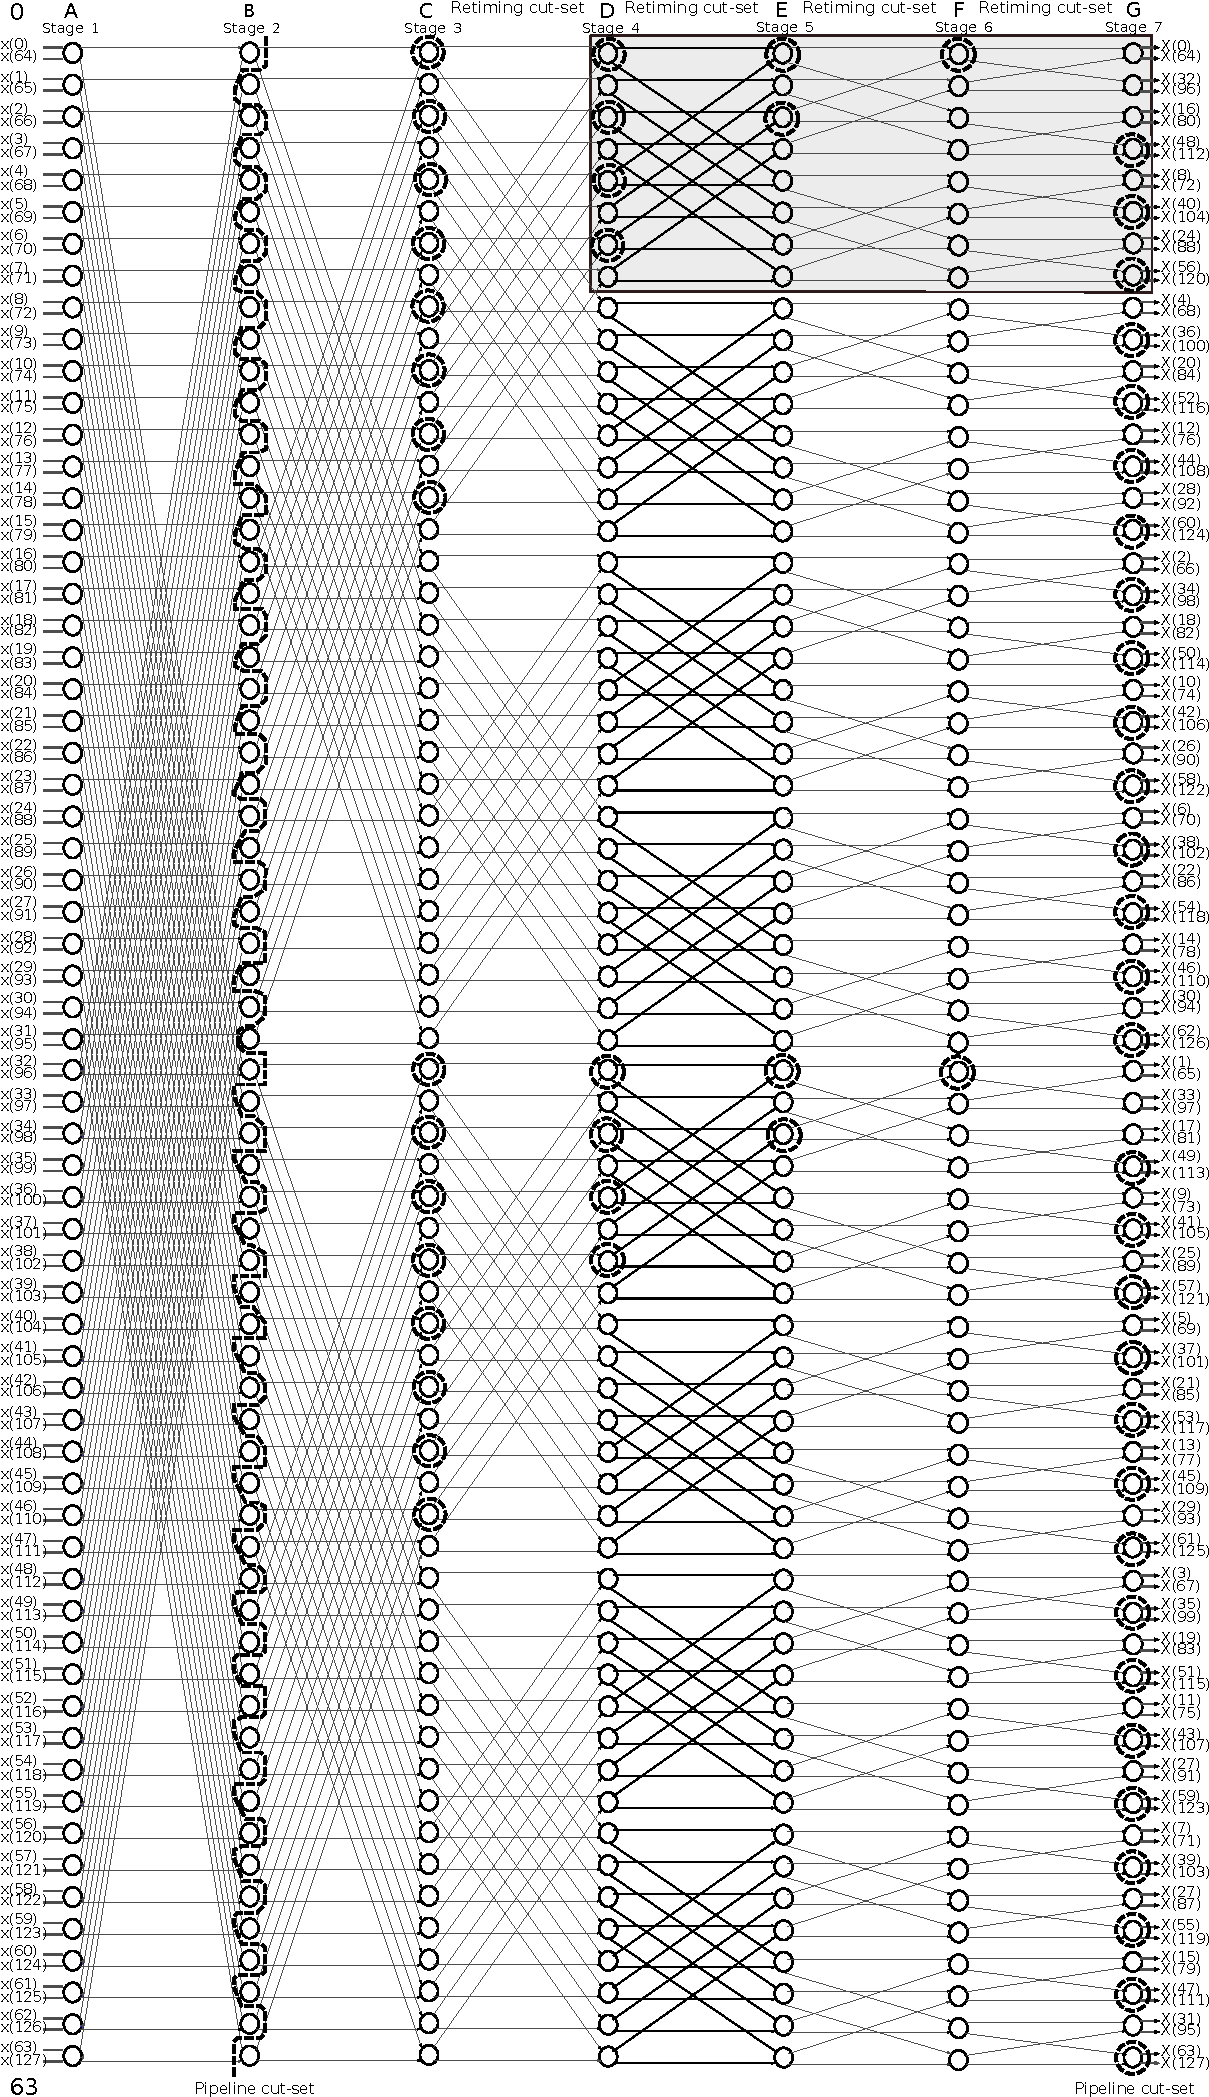
\includegraphics[width=\linewidth]{Diagramas/miSeccionFiguras/128puntosRadix8BurbujasPipelined_Kevin.pdf}
\caption{Pipelined DFG of a 128-point DIF FFT as a preprocessing step for folding.}
\label{fig:pipe_dfg_128}
\end{figure}
\begin{figure*}[!t]
	\centering
	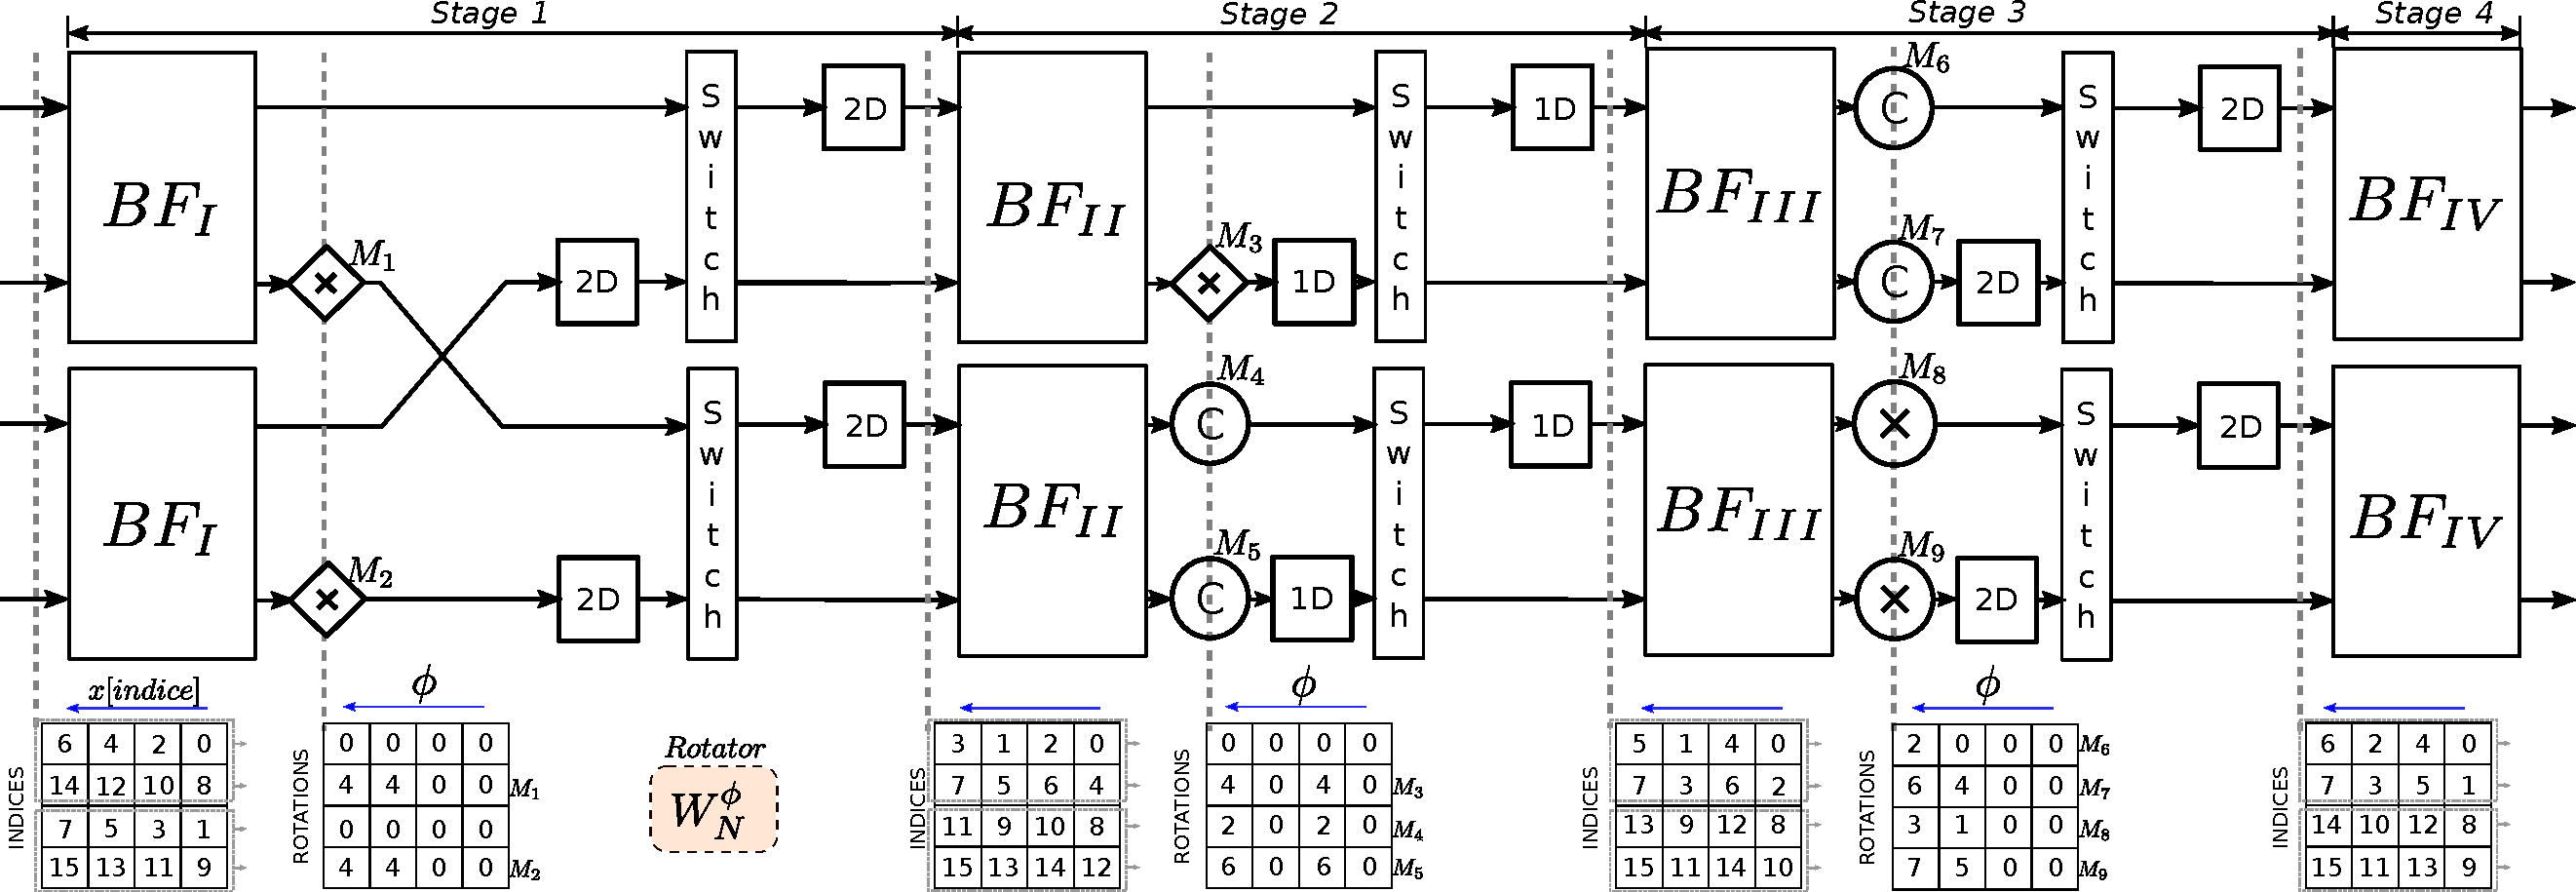
\includegraphics[width=0.75\linewidth]{Diagramas/miSeccionFiguras/4Paralelo16pRadix8.pdf}
	\caption{Folding architecture for the computation of a radix-$2^3$ 16-point DIF complex FFT.}
	\label{fig:circ-folding-16}
\end{figure*}
\begin{small}
\begin{table*}[t!]
	\centering
	\begin{threeparttable}
		\centering
		\caption{Folding set for the DFG showed in Fig. \ref{fig:pipe_dfg_128}}
		\label{tab:fold_set_128} 
		\begin{tabular}{|c||cccccccccccccccc|}
			\hline
			\multirow{2}{*}{A} & A0 & A2 & A4 & A6 & A8 & A10 & A12 & A14 & A16 & A18 & A20 & A22 & A24 & A26 & A28 & A30 \\  
			& A32 & A34 & A36 & A38 & A40 & A42 & A44 & A46 & A48 & A50 & A52 & A54 & A56 & A58 & A60 & A62 \\  
			\hline
			\multirow{2}{*}{A'} & A1 & A3 & A5 & A7 & A9 & A11 & A13 & A15 & A17 & A19 & A21 & A23 & A25 & A27 & A29 & A31 \\  
			& A33 & A35 & A37 & A39 & A41 & A43 & A45 & A47 & A49 & A51 & A53 & A55 & A57 & A59 & A61 & A63 \\  
			\hline
			\multirow{2}{*}{B} & B1 & B3 & B5 & B7 & B9 & B11 & B13 & B15 & B17 & B19 & B21 & B23 & B25 & B27 & B29 & B31 \\  
			& B0 & B2 & B4 & B6 & B8 & B10 & B12 & B14 & B16 & B18 & B20 & B22 & B24 & B26 & B28 & B30 \\  
			\hline
			\multirow{2}{*}{B'} & B33 & B35 & B37 & B39 & B41 & B43 & B45 & B47 & B49 & B51 & B53 & B55 & B57 & B59 & B61 & B63 \\  
			& B32 & B34 & B36 & B38 & B40 & B42 & B44 & B46 & B48 & B50 & B52 & B54 & B56 & B58 & B60 & B62 \\  
			\hline
			\multirow{2}{*}{C} & C16 & C18 & C20 & C22 & C24 & C26 & C28 & C30 & C1 & C3 & C5 & C7 & C9 & C11 & C13 & C15 \\  
			& C17 & C19 & C21 & C23 & C25 & C27 & C29 & C31 & C0 & C2 & C4 & C6 & C8 & C10 & C12 & C14 \\  
			\hline
			\multirow{2}{*}{C'} & C48 & C50 & C52 & C54 & C56 & C58 & C60 & C62 & C33 & C35 & C37 & C39 & C41 & C43 & C45 & C47 \\  
			& C49 & C51 & C53 & C55 & C57 & C59 & C61 & C63 & C32 & C34 & C36 & C38 & C40 & C42 & C44 & C46 \\  
			\hline
			\multirow{2}{*}{D} & D8 & D10 & D12 & D14 & D16 & D18 & D20 & D22 & D24 & D26 & D28 & D30 & D1 & D3 & D5 & D7 \\  
			& D9 & D11 & D13 & D15 & D17 & D19 & D21 & D23 & D25 & D27 & D29 & D31 & D0 & D2 & D4 & D6 \\  
			\hline
			\multirow{2}{*}{D'} & D40 & D42 & D44 & D46 & D48 & D50 & D52 & D54 & D56 & D58 & D60 & D62 & D33 & D35 & D37 & D39 \\  
			& D41 & D43 & D45 & D47 & D49 & D51 & D53 & D55 & D57 & D59 & D61 & D63 & D32 & D34 & D36 & D38 \\  
			\hline
			\multirow{2}{*}{E} & E4 & E6 & E8 & E10 & E12 & E14 & E16 & E18 & E20 & E22 & E24 & E26 & E28 & E30 & E1 & E3 \\  
			& E5 & E7 & E9 & E11 & E13 & E15 & E17 & E19 & E21 & E23 & E25 & E27 & E29 & E31 & E0 & E2 \\  
			\hline
			\multirow{2}{*}{E'} & E36 & E38 & E40 & E42 & E44 & E46 & E48 & E50 & E52 & E54 & E56 & E58 & E60 & E62 & E33 & E35 \\  
			& E37 & E39 & E41 & E43 & E45 & E47 & E49 & E51 & E53 & E55 & E57 & E59 & E61 & E63 & E32 & E34 \\  
			\hline
			\multirow{2}{*}{F} & F2 & F4 & F6 & F8 & F10 & F12 & F14 & F16 & F18 & F20 & F22 & F24 & F26 & F28 & F30 & F1 \\  
			& F3 & F5 & F7 & F9 & F11 & F13 & F15 & F17 & F19 & F21 & F23 & F25 & F27 & F29 & F31 & F0 \\  
			\hline
			\multirow{2}{*}{F'} & F34 & F36 & F38 & F40 & F42 & F44 & F46 & F48 & F50 & F52 & F54 & F56 & F58 & F60 & F62 & F33 \\  
			& F35 & F37 & F39 & F41 & F43 & F45 & F47 & F49 & F51 & F53 & F55 & F57 & F59 & F61 & F63 & F32 \\  
			\hline
			\multirow{2}{*}{G} & G3 & G5 & G7 & G9 & G11 & G13 & G15 & G17 & G19 & G21 & G23 & G25 & G27 & G29 & G31 & G0 \\  
			& G2 & G4 & G6 & G8 & G10 & G12 & G14 & G16 & G18 & G20 & G22 & G24 & G26 & G28 & G30 & G1 \\  
			\hline
			\multirow{2}{*}{G'} & G35 & G37 & G39 & G41 & G43 & G45 & G47 & G49 & G51 & G53 & G55 & G57 & G59 & G61 & G63 & G32 \\  
			& G34 & G36 & G38 & G40 & G42 & G44 & G46 & G48 & G50 & G52 & G54 & G56 & G58 & G60 & G62 & G33 \\
			\hline
		\end{tabular}
	\end{threeparttable}
\end{table*}
\end{small}
\begin{figure*}[!t]
	\centering
	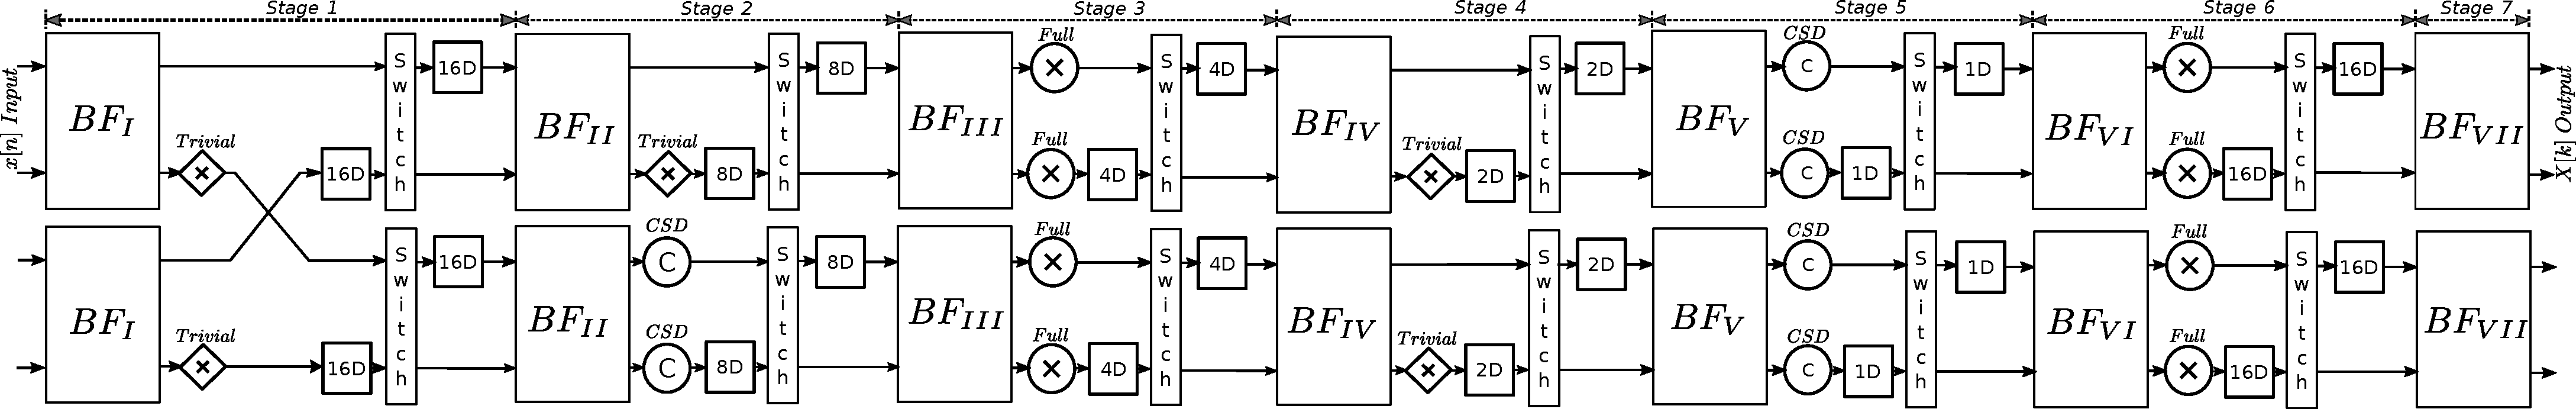
\includegraphics[width=1.0\linewidth]{Diagramas/miSeccionFiguras/4Paralelo128pRadix8.pdf}
	\caption{Folding architecture for the computation of a radix-$2^3$ 128-point DIF complex FFT.}
	\label{fig:circ-folding-128}
\end{figure*}
%\begin{figure*}[t!]
%	\centering
%	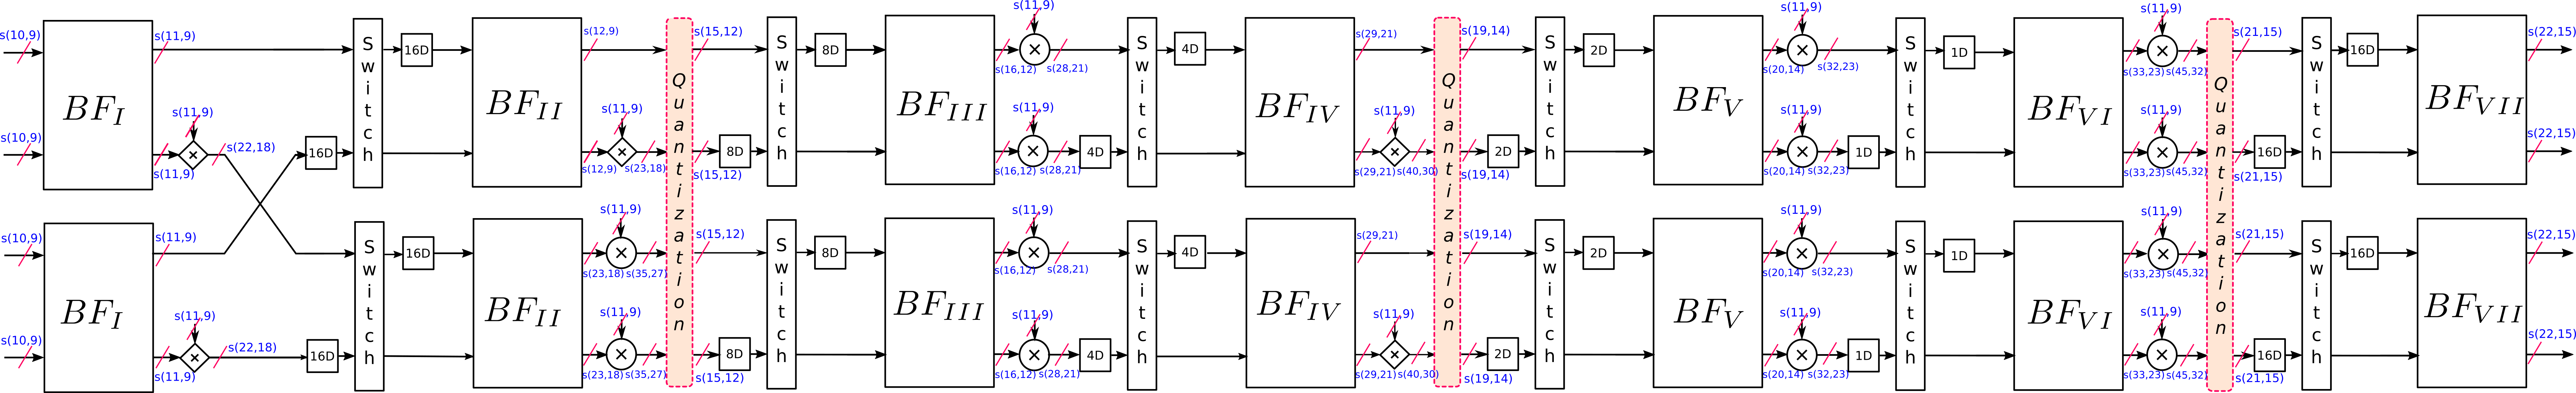
\includegraphics[width=\linewidth]{Diagramas/miSeccionFiguras/4Paralelo128pRadix8Cuantizacion1}
%	\caption{Quantization for a 128-point 4-parallel pipelined complex FFT architecture}
%	\label{fig:4paralelo128pradix8cuantizacion1}
%\end{figure*}



%%%%%%%%%%
%% Seccion
%%%%%%%%%%
\section{IMPLEMENTATION}
In this section we are going to begin with the process of how accomplish the implementation of our 4-parallel architecture for the computation of 128-point \textit{radix}-$2^3$ DIF complex FFT.
First, we wrote a \textit{MATLAB} simulator to validate the operation of our design and the design presented in \cite{garrido_pipelined_2013,garrido_feedforward_2018}. Therefore, we can have a reference architecture for compare the design that we deduce. After that, we take all these information to generate a Synthesizable \textit{Verilog} code with different levels of optimizations with a powerful tool like \textit{Synopsys} to get a final design integrated of Standard Cells $@45nm$.
%%%%%%%%%%%%%
%% Subseccion
%%%%%%%%%%%%%
\subsection{Floating and Fixed point Simulator}
\begin{figure*}[t!]
	\centering
	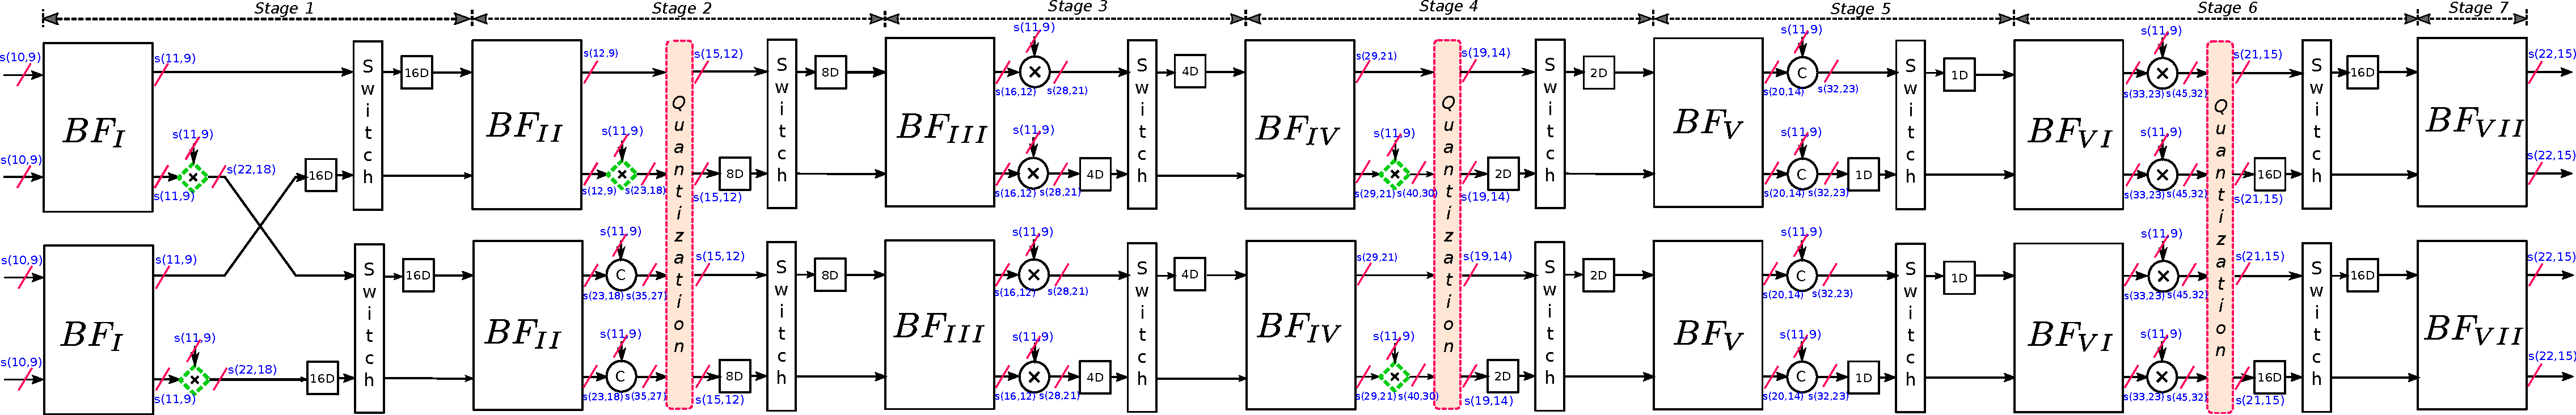
\includegraphics[width=\linewidth]{Diagramas/miSeccionFiguras/4Paralelo128pRadix8Cuantizacion1.pdf}
	\caption{Quantization for a 128-point 4-parallel pipelined complex FFT architecture}
	\label{fig:4paralelo128pradix8cuantizacion1}
\end{figure*}
\begin{figure}[t!]
	\centering
	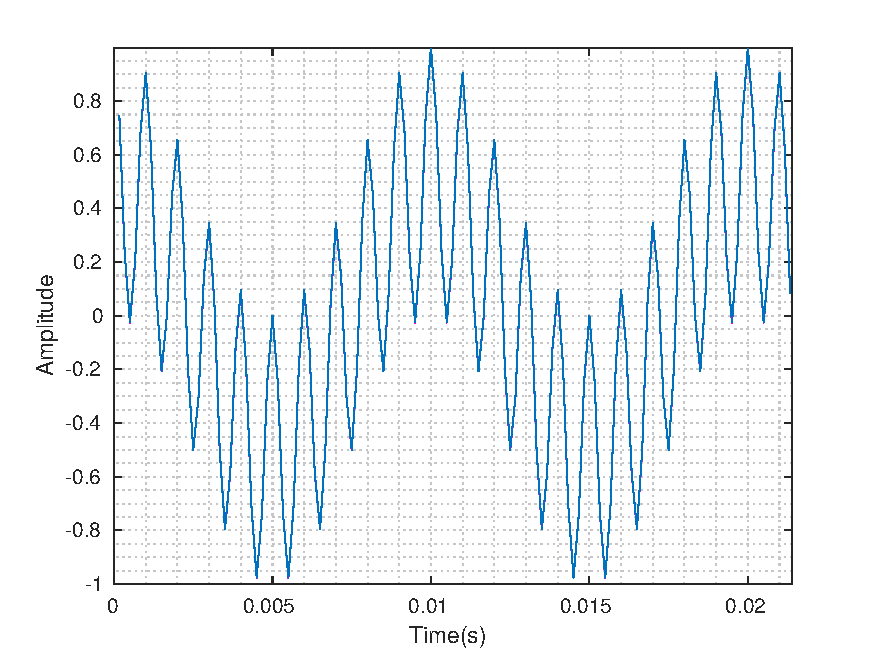
\includegraphics[width=0.92\linewidth]{Diagramas/DftInputSignal.pdf}
	\caption{Input signal $x[n]$ in time domain}
	\label{fig:dftinputsignal}
\end{figure}
\begin{figure}[t!]
	\centering
	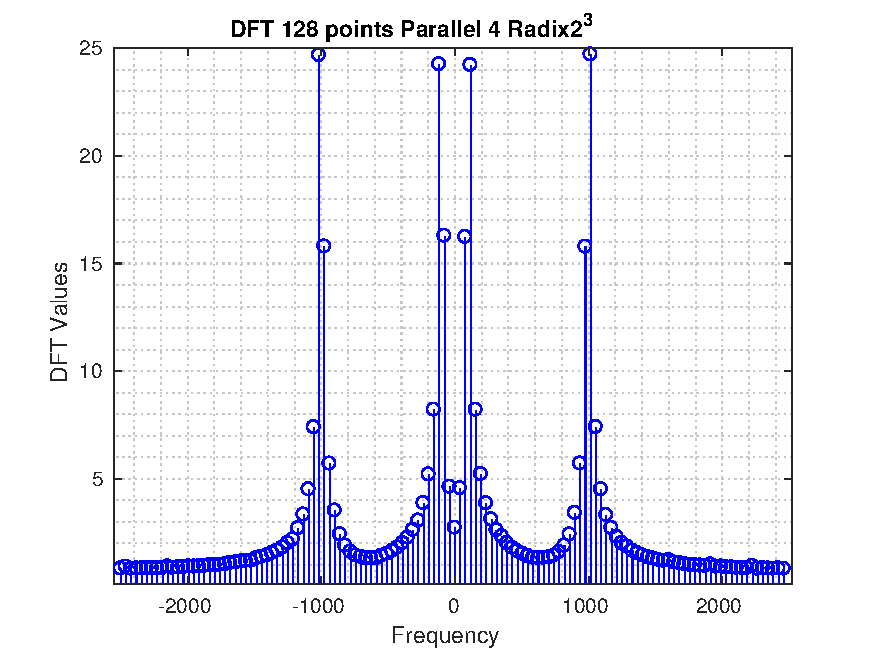
\includegraphics[width=0.95\linewidth]{Diagramas/DftFixedPoint.pdf}
	\caption{Output samples, absolute value vs frequency $|X[k]|$}
	\label{fig:dftfixedpoint}
\end{figure}
The input signal Fig. \ref{fig:dftinputsignal} to our architecture will be a mixture of sinusoid signals with two frequency values, theses signal will be normalizing to the unity and in this way we can have a test bench design.
\begin{align}\label{eq: inputSignal}
x'[n] &= cos(2\pi f_1 n T_s) + cos(2\pi f_2 n T_s)  \\
x[n] &= x'[n]/max\{x'[n]\} 						\nonumber
\end{align}
where $f_1=100Hz$, $f_2=1000Hz$ and $T_s$ is the sampled period.

In each stage of the Fig. \ref{fig:4paralelo128pradix8cuantizacion1}, input samples that propagate stage by stage will be carefully quantized with the purpose of getting a high SQNR (Signal to Quantization Noise Ratio).
\begin{equation*}%\label{eq:sqnr}
SQNR_{dB} = 10log_{10} \bigg(  \frac{  Var\{Signal_{FloatPoint}\}  }{  Var\{Signal_{FloatPoint} - Signal_{FixedPoint}\}}  \bigg)
\end{equation*}
SQNR represents computing the logarithmic relationship between float signal variance over error variance from an signal given.

The input signal $x[n]$ is quantized with a value of $S(10,9)$, that representation means a number signed (S) with $10$ total bits and $9$ fractional bits. The value calculated of SQNR for the input is $56.9dB$. Following the same steps, we can compute the SQNR for the \textit{twiddle} factors and the architecture's output.

Twiddles factor are quantized with a relation of $S(11,9)$ and the complex output signal $X[k]$ with $S(22,15)$. Output quantization for the real part is $46.8dB$ and for the imaginary part $47.3dB$. In general, a value of quantization close to $50dB$ is a good approximation. Out signal from our \textit{MATLAB} fixed-point model from the architecture in Fig. \ref{fig:4paralelo128pradix8cuantizacion1} the output signal is given in Fig. \ref{fig:dftfixedpoint}, that represents a first approach in our calculation of a DFT without optimization.
\begin{figure}[t!]
	\centering
	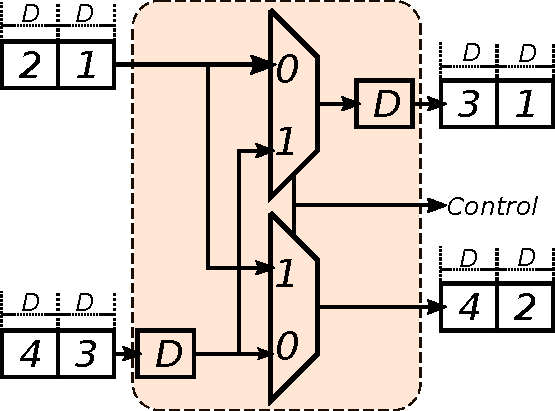
\includegraphics[width=0.42\linewidth]{Diagramas/miSeccionFiguras/Shift.pdf}
	\caption{Circuit for data shuffling}
	\label{fig:shift}
\end{figure}
\begin{figure}[t!]
	\centering
	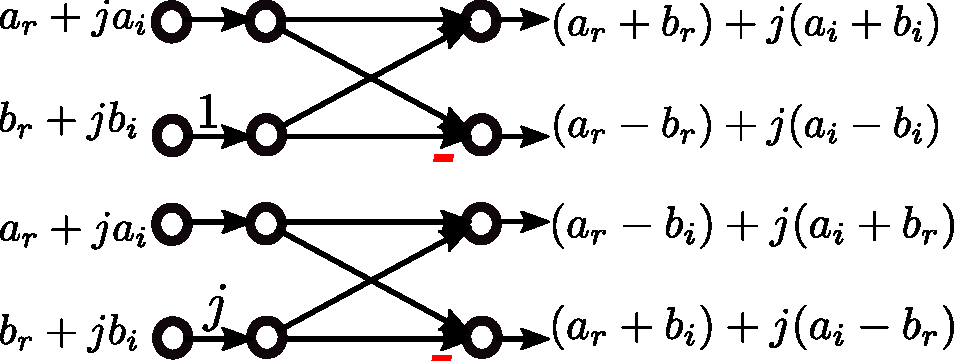
\includegraphics[width=0.65\linewidth]{Diagramas/miSeccionFiguras/ButterComplejo.pdf}
	\caption{Complex butterfly }
	\label{fig:buttercomplejo}
\end{figure}
\begin{figure}[t!]
	\centering
	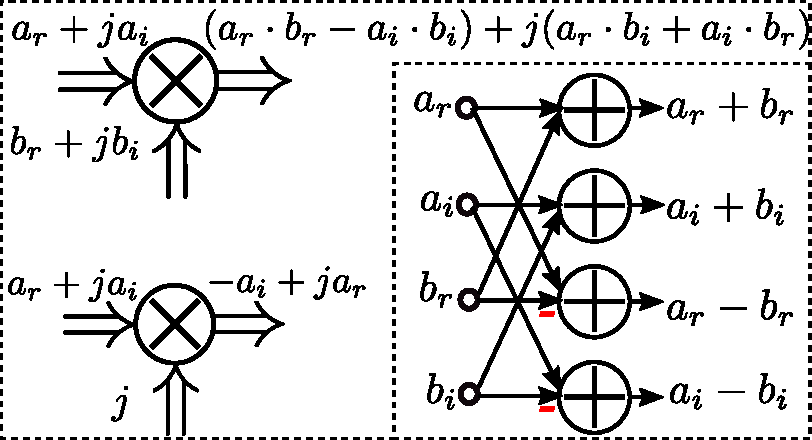
\includegraphics[width=0.65\linewidth]{Diagramas/miSeccionFiguras/SumMult.pdf}
	\caption{Complex multiplier and complex adder}
	\label{fig:summult}
\end{figure}

The combination between latencies (delays registers) and switches in all stages in Fig. \ref{fig:4paralelo128pradix8cuantizacion1} is the equivalent circuit shows in Fig. \ref{fig:shift}, that is used to appropriately order samples in each butterflies input.

Whole elements on the architecture such as multipliers and butterflies are complex as Fig. \ref{fig:buttercomplejo} and \ref{fig:summult}. On an implementation is essential divide the signal in its real and imaginary part with the purpose of process them independently. A \textit{general rotator} (full complex multiplier) generate a real and imaginary component that is composed by a real multiplication an one addition, but a \textit{trivial rotator} only change the components of a complex signal. These relations are important at the moment of doing the quantization process to ensure an appropriate quantity of bits.
%%%%%%%%%%%%%
%% Subseccion
%%%%%%%%%%%%%
\subsection{Verilog (HDL) Model} 
\begin{figure*}[t!]
	\centering
	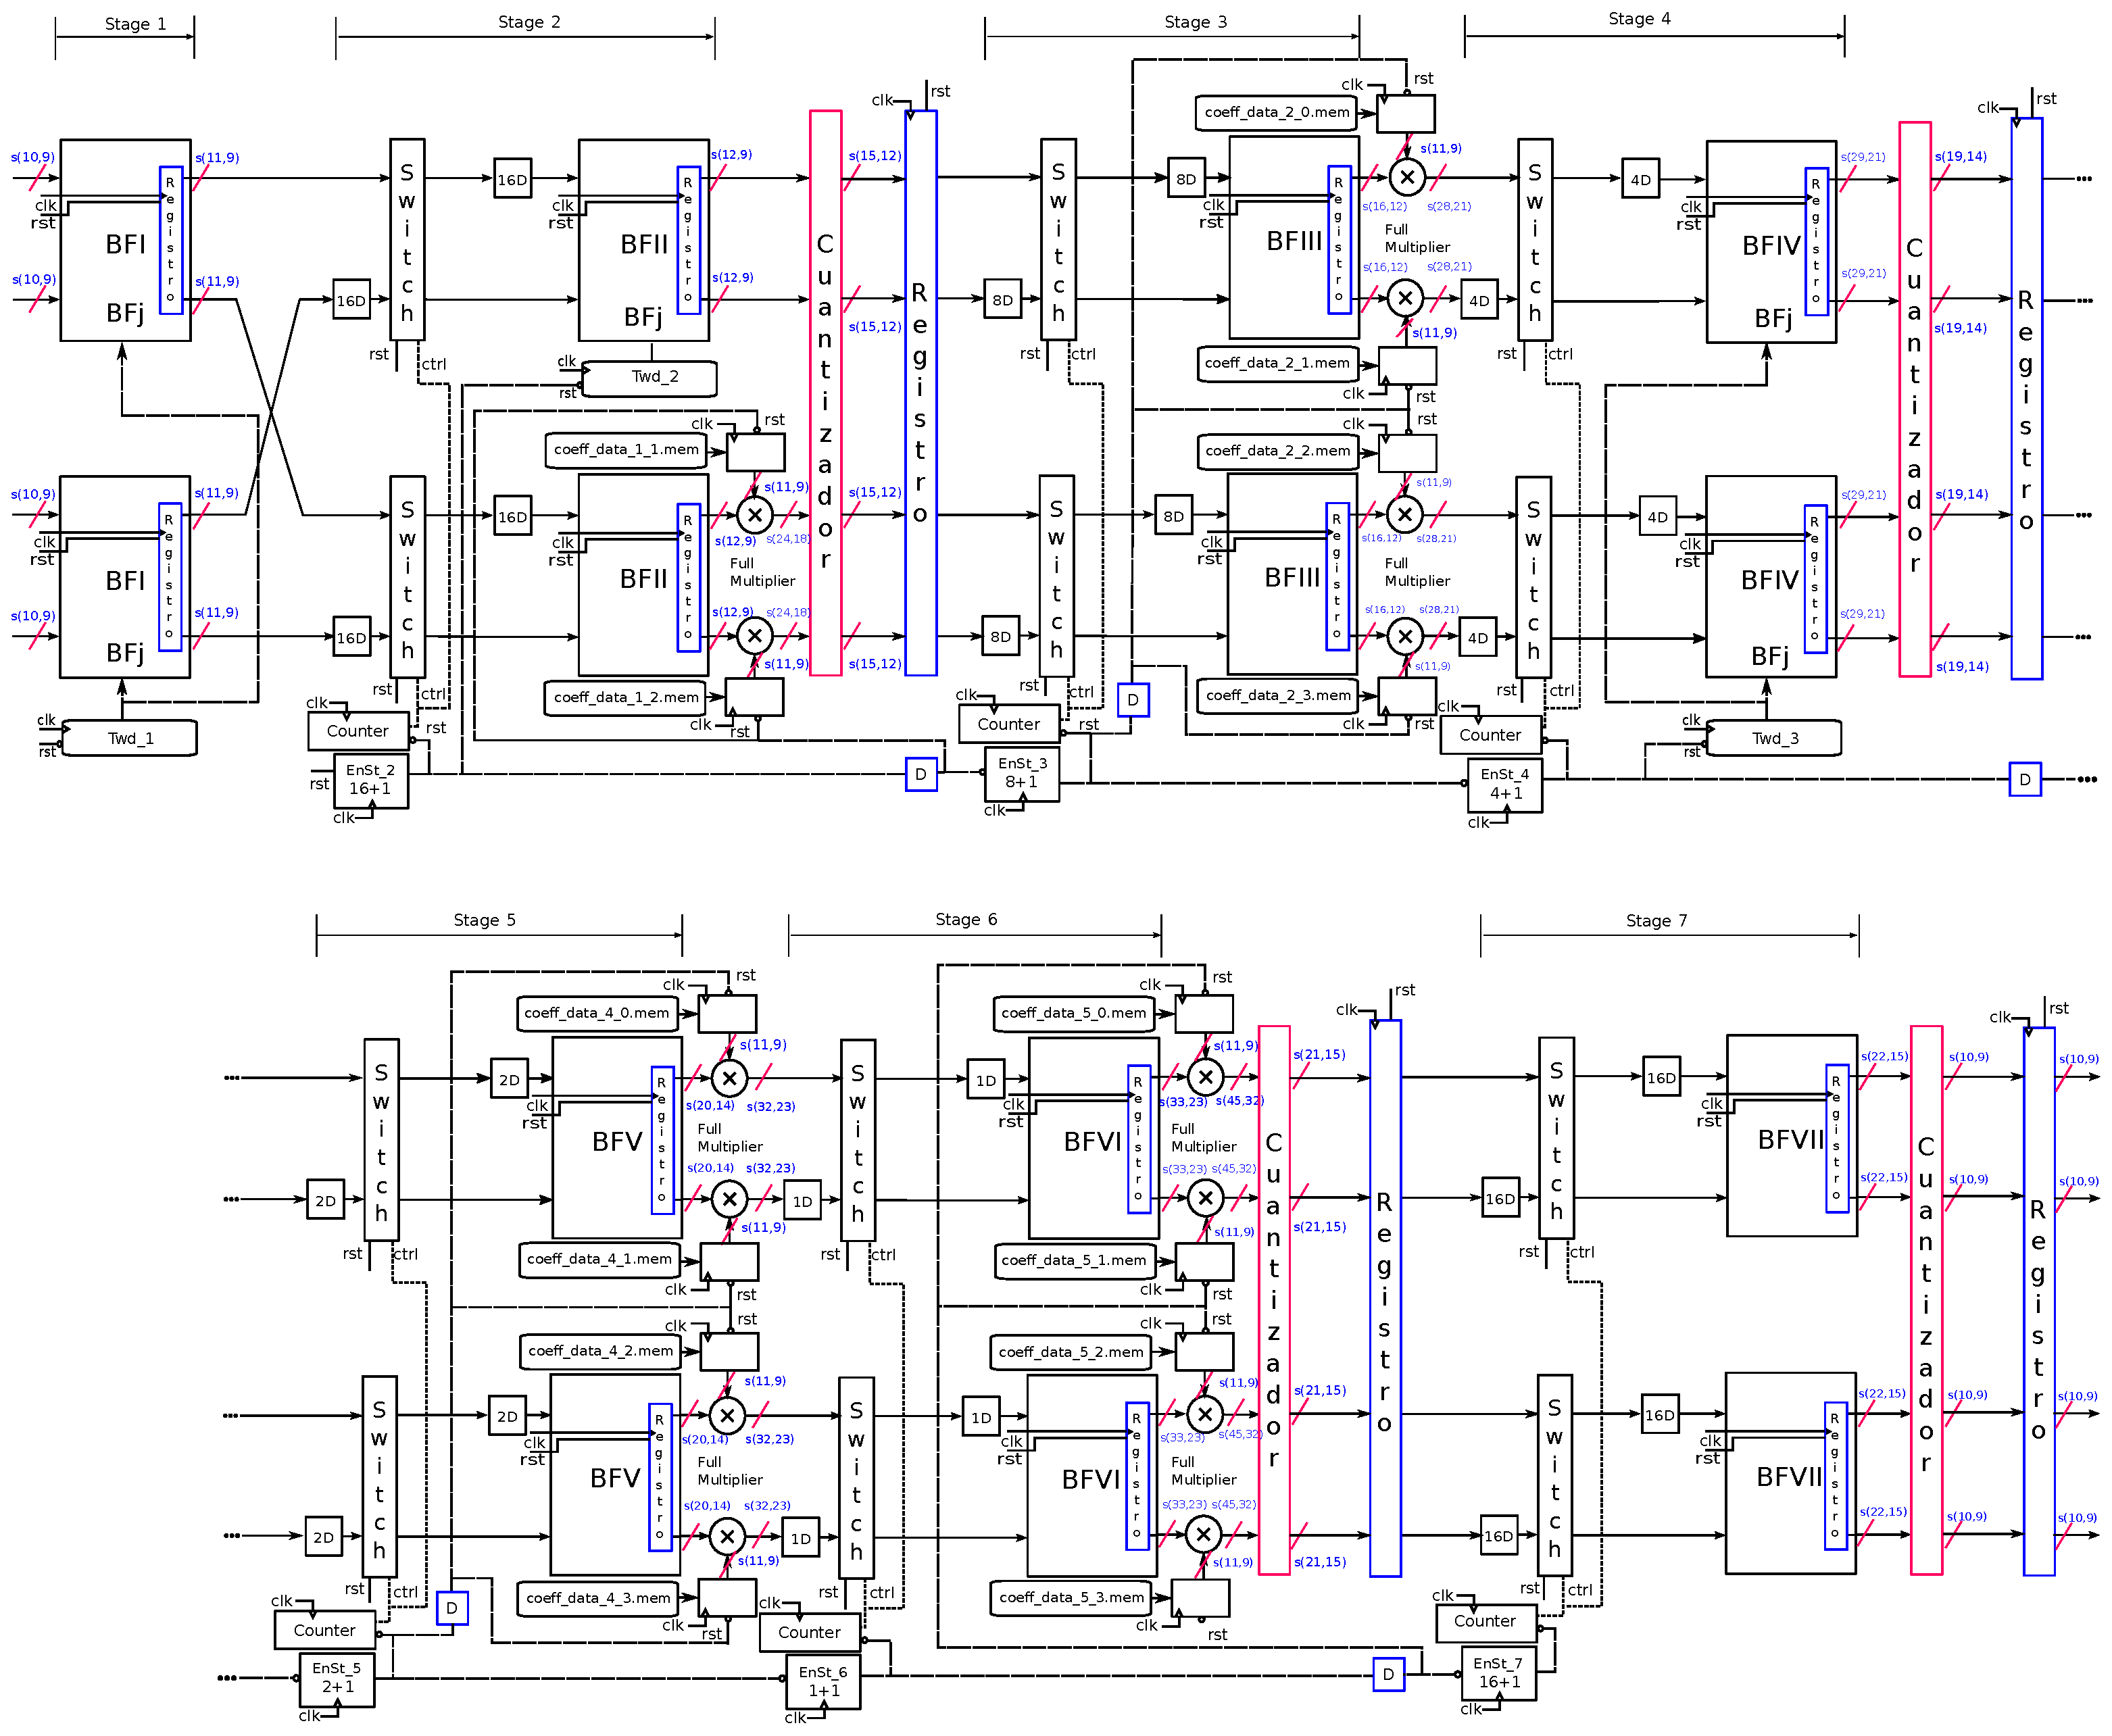
\includegraphics[width=\linewidth]{Diagramas/V5_esquema_p.eps}
	\caption{RTL (Register transfer level) design for a 4-parallel \textit{radix}-$2^3$ 128-point DIF FFT with Optimization}
	\label{fig:v5esquemap}
\end{figure*}

Hello wold!



%%%%%%%%%%
%% Seccion
%%%%%%%%%%
\section{RESULTS}



%%%%%%%%%%
%% Seccion
%%%%%%%%%%
\section{CONCLUSION}



%%%%%%%%%%%%%%
% Bibliografia
%%%%%%%%%%%%%%
\bibliographystyle{IEEEtran}
\bibliography{referenciasFFT}
%%%%%%%%
% FIN
%%%%%%%%
\end{document}
